\documentclass{beamer}
 
\usepackage[utf8]{inputenc}
\usepackage[english]{babel}
\usepackage{amsmath}
\usepackage{amsfonts}
\usepackage{amssymb}
\usepackage{graphicx} 
\usepackage{latexsym} 
\usepackage{listings}
\usepackage{xcolor}
\usepackage{soul}
\usepackage[T1]{fontenc}
\usepackage{amsthm}
\usepackage{mathtools}
\usepackage{setspace}
\usepackage{array,multirow,makecell}
\usepackage{geometry}
\usepackage{textcomp}
\usepackage{float}
\usepackage{bbold}
\usepackage{wrapfig}
\usepackage{textpos}

\rmfamily

\usetheme{Madrid}
%%\usecolortheme{beaver}



\title{LP 45 Paramagnétisme, ferromagnétisme : approximation du champ moyen}
\author{Naïmo Davier}
\institute{Université Paul sabatier}

 
\begin{document}
	
\begin{frame}
	\titlepage
\end{frame}

\addtocounter{framenumber}{-1}
\title{LP 45 Para, ferro}

\begin{frame}
\frametitle{Paramagnétisme, aimantation spin 1/2}
\centerline{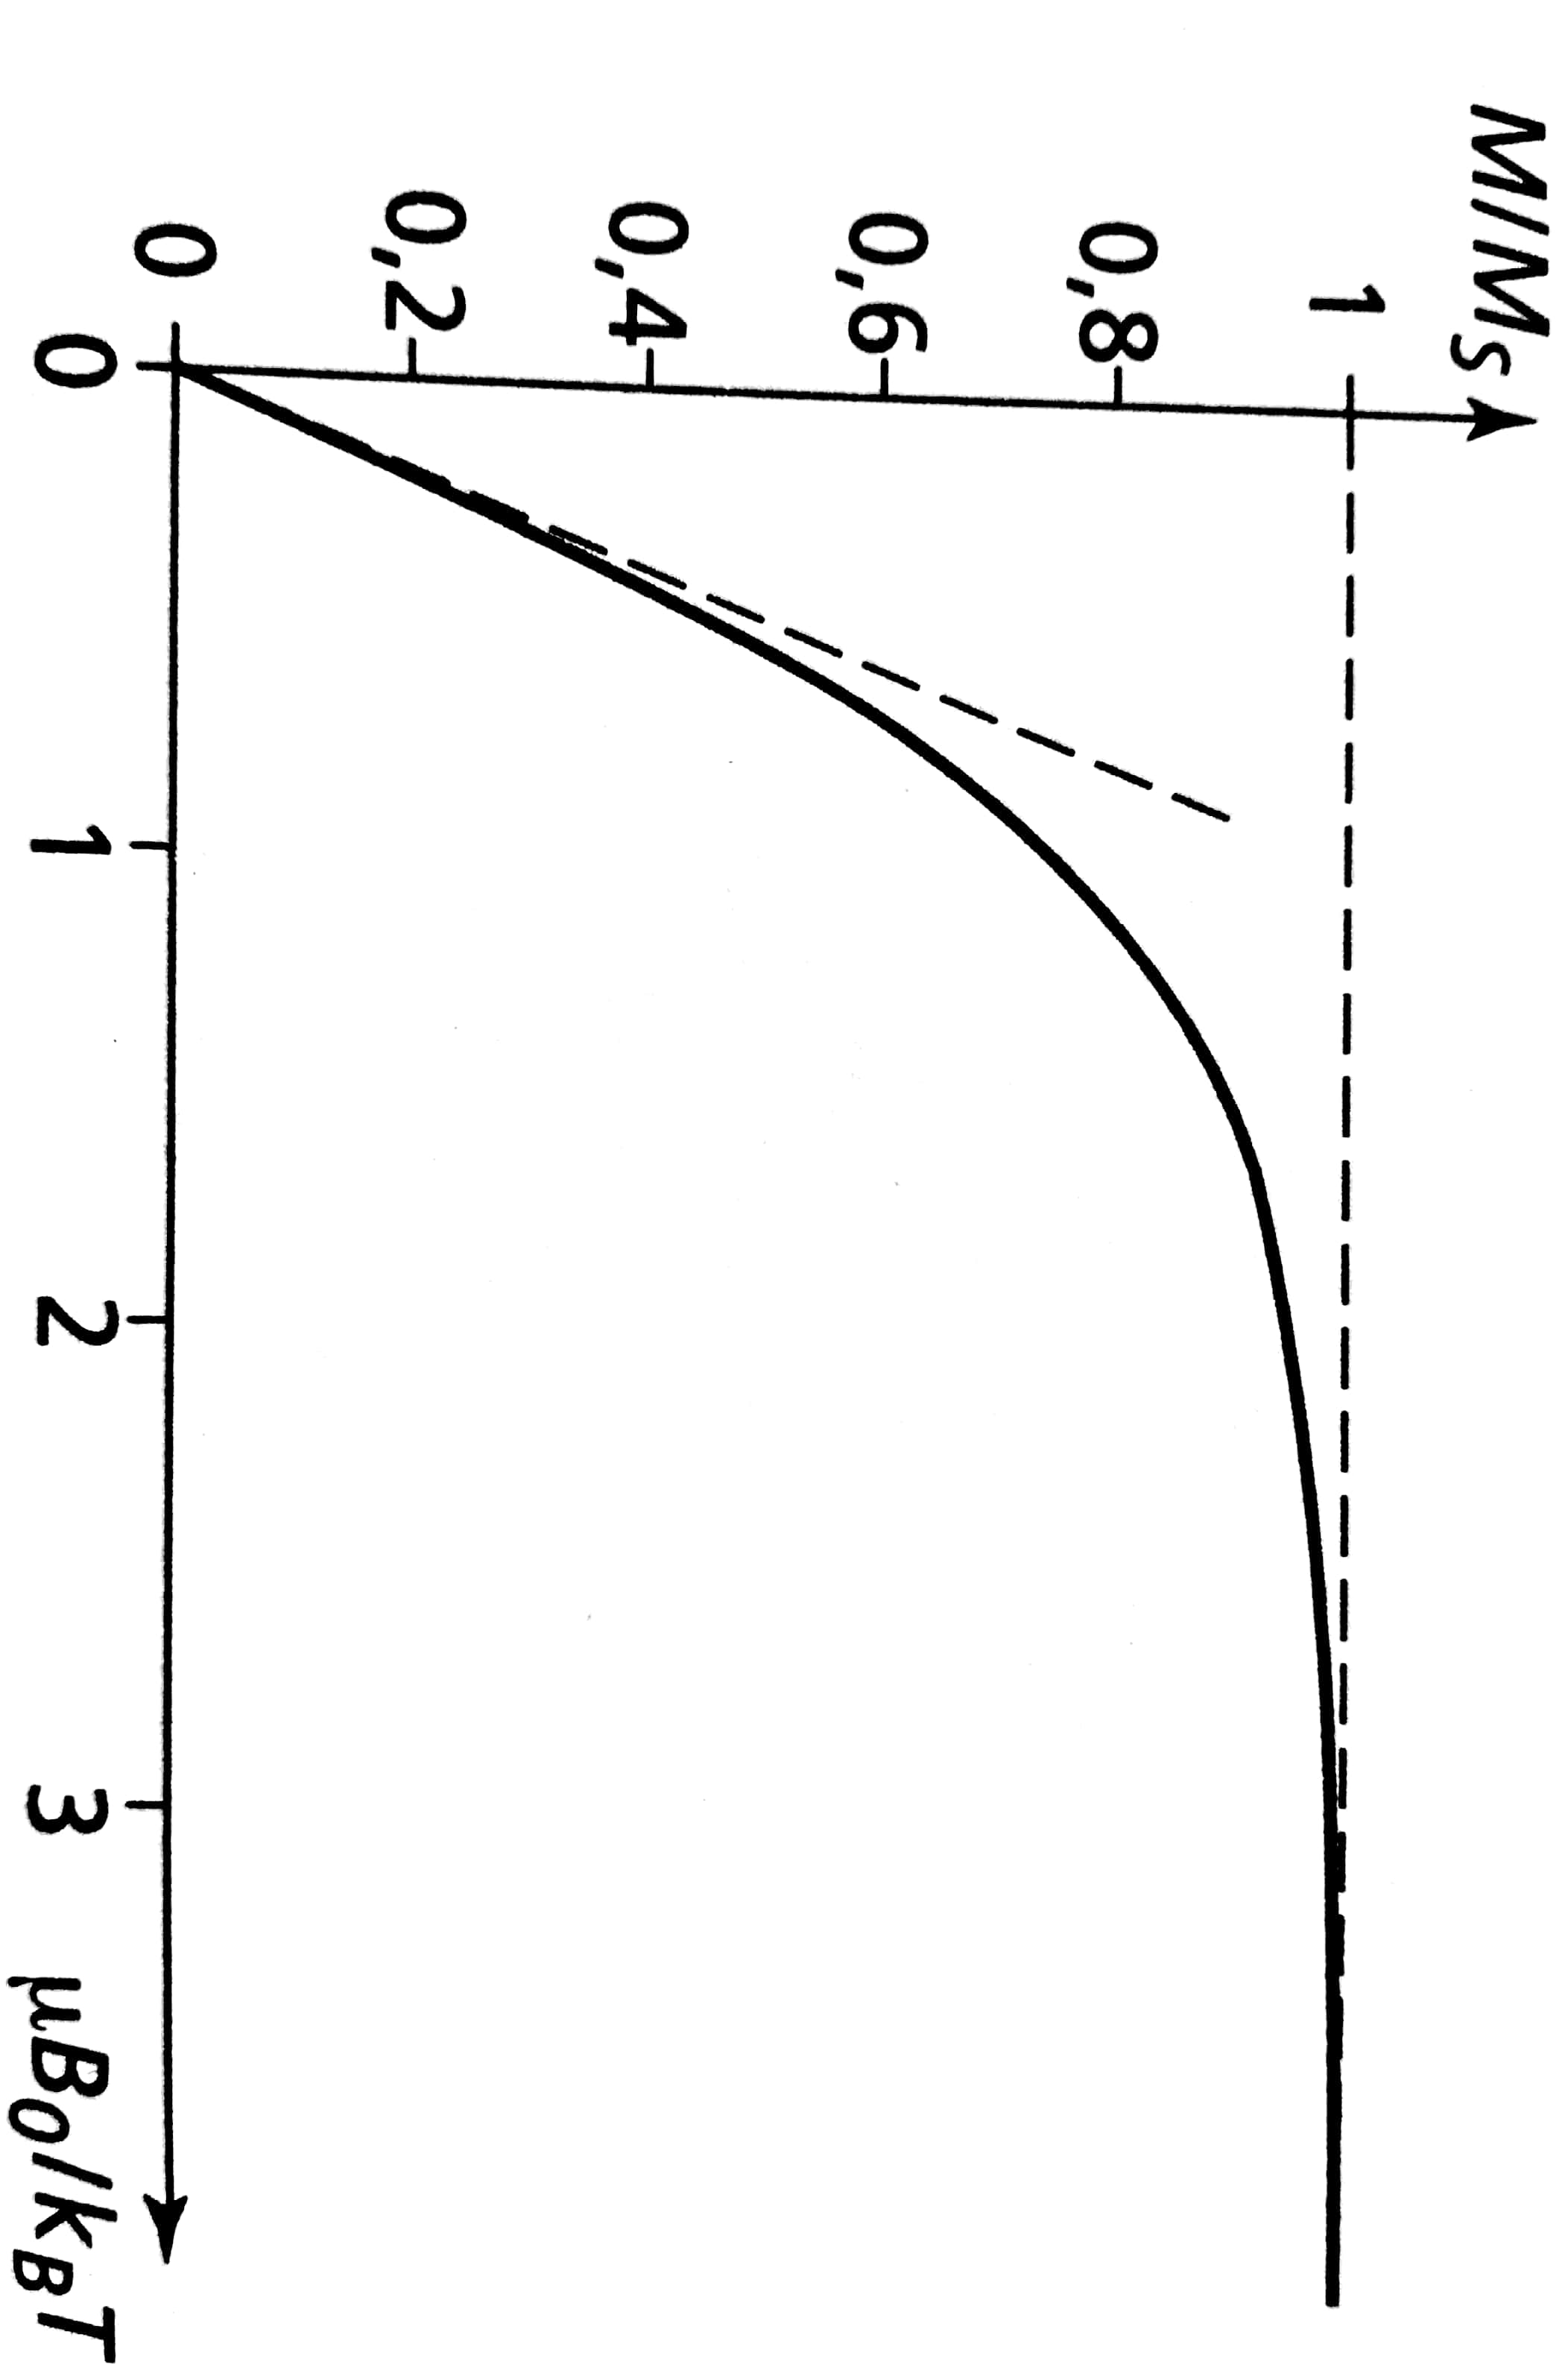
\includegraphics[width=6cm,angle=90]{para}}
\end{frame}

\begin{frame}
\frametitle{Paramagnétisme, aimantation cas général $J\neq1/2$}
\centerline{\includegraphics[width=11.5cm]{cas_j_n0,5}}
\end{frame}

\begin{frame}
\frametitle{Ferromagnétisme, cycle d'hystérésis}
\begin{figure}[h]
	\centerline{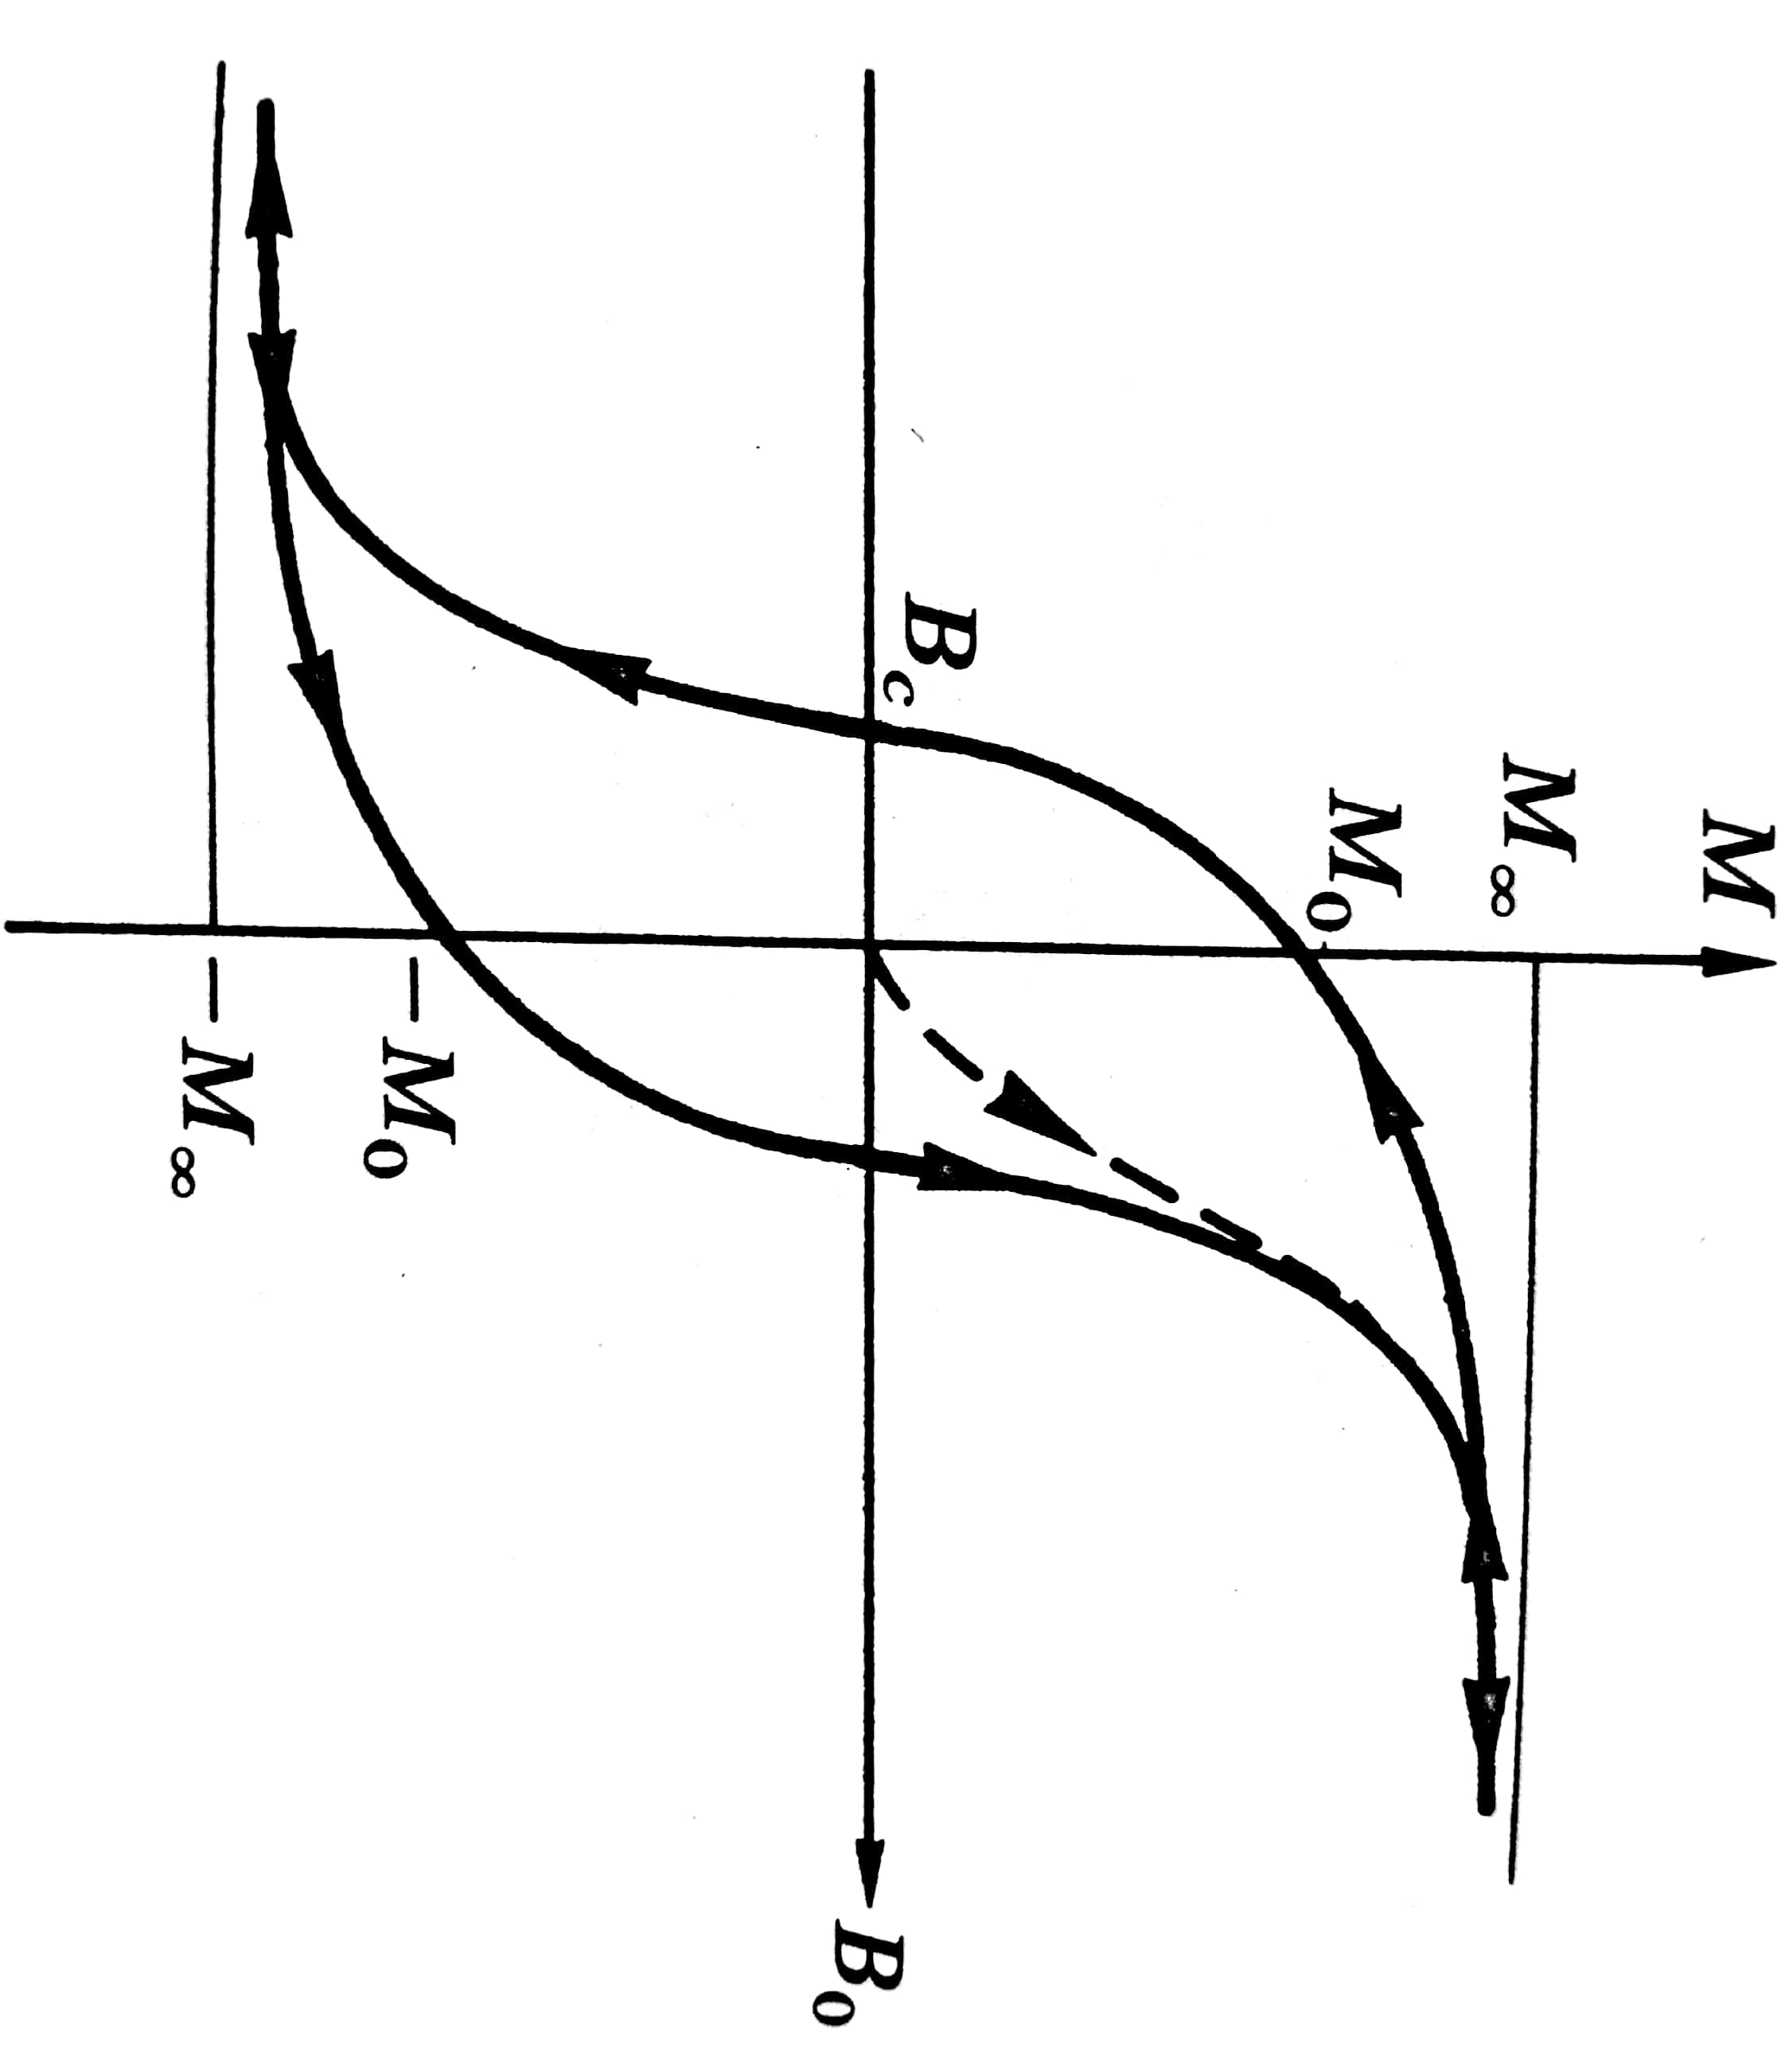
\includegraphics[width=7cm, angle=90]{hysteresis}}
\end{figure}
\end{frame}

\begin{frame}
\frametitle{Ferromagnétisme : domaines de Weiss}
\begin{figure}[h]
	\centerline{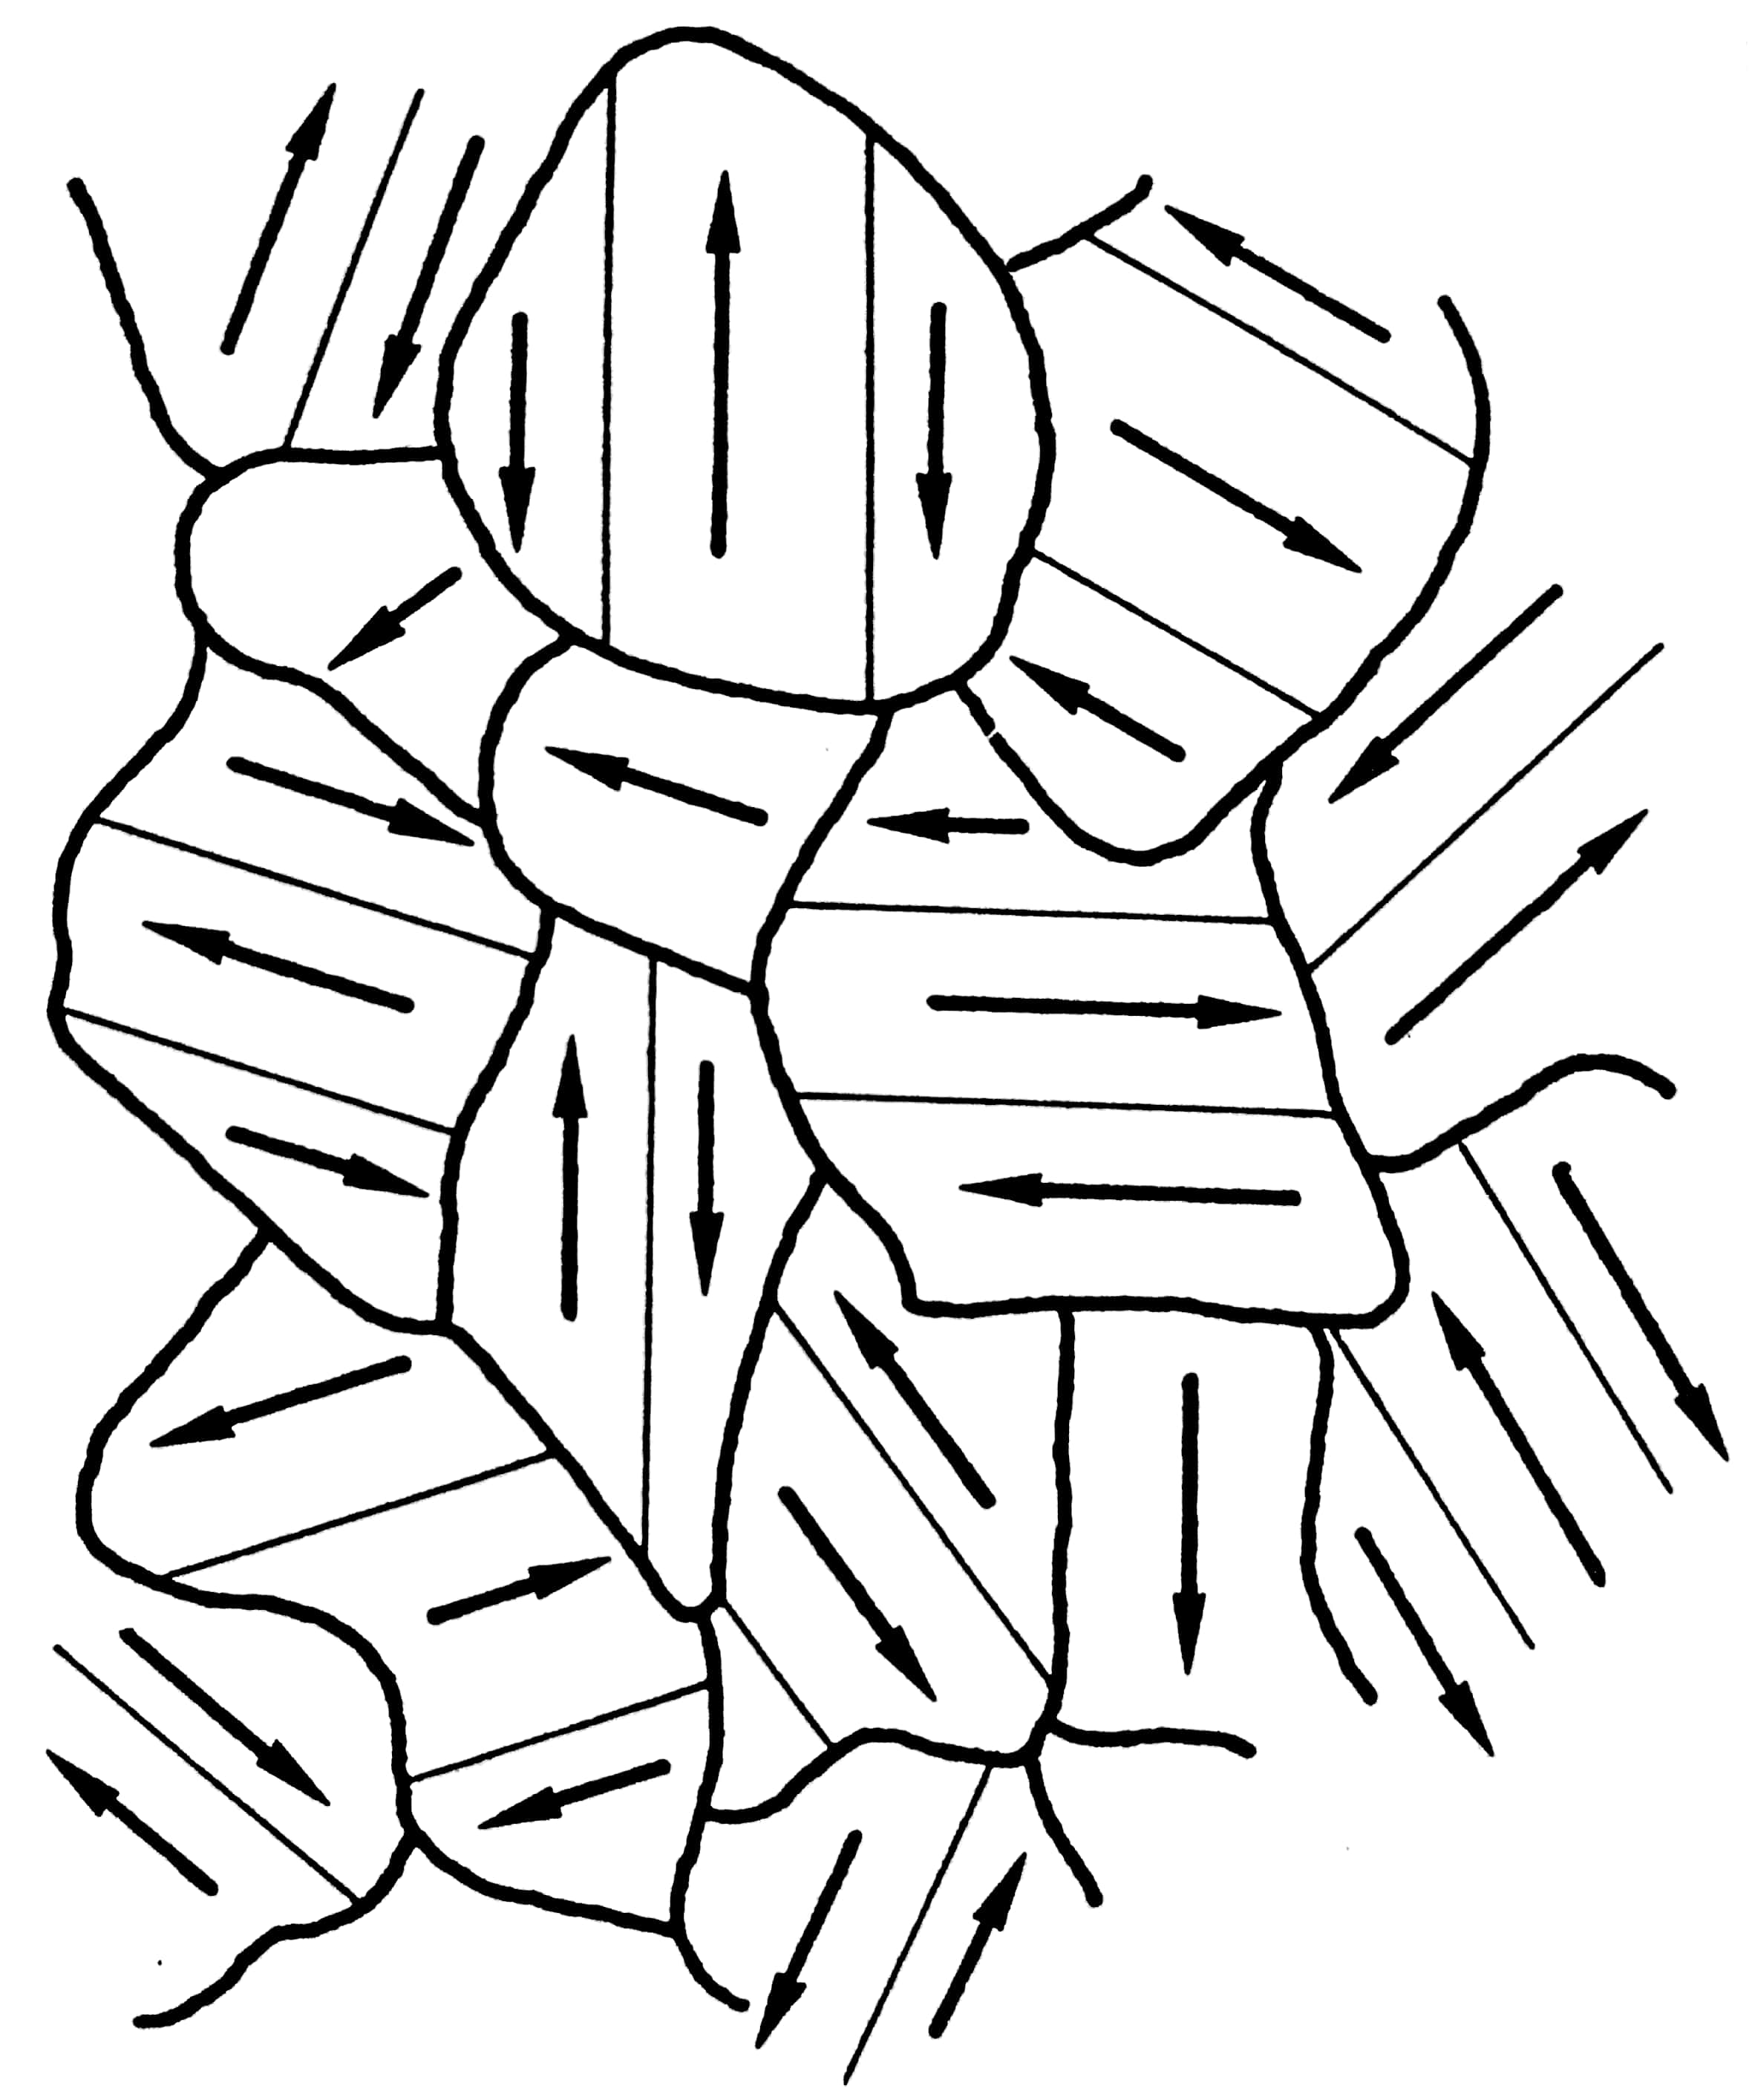
\includegraphics[width=7cm,angle=90]{weiss}}
\end{figure}
\end{frame}

\begin{frame}
\frametitle{Solution en champ nul}
\begin{figure}
	\centerline{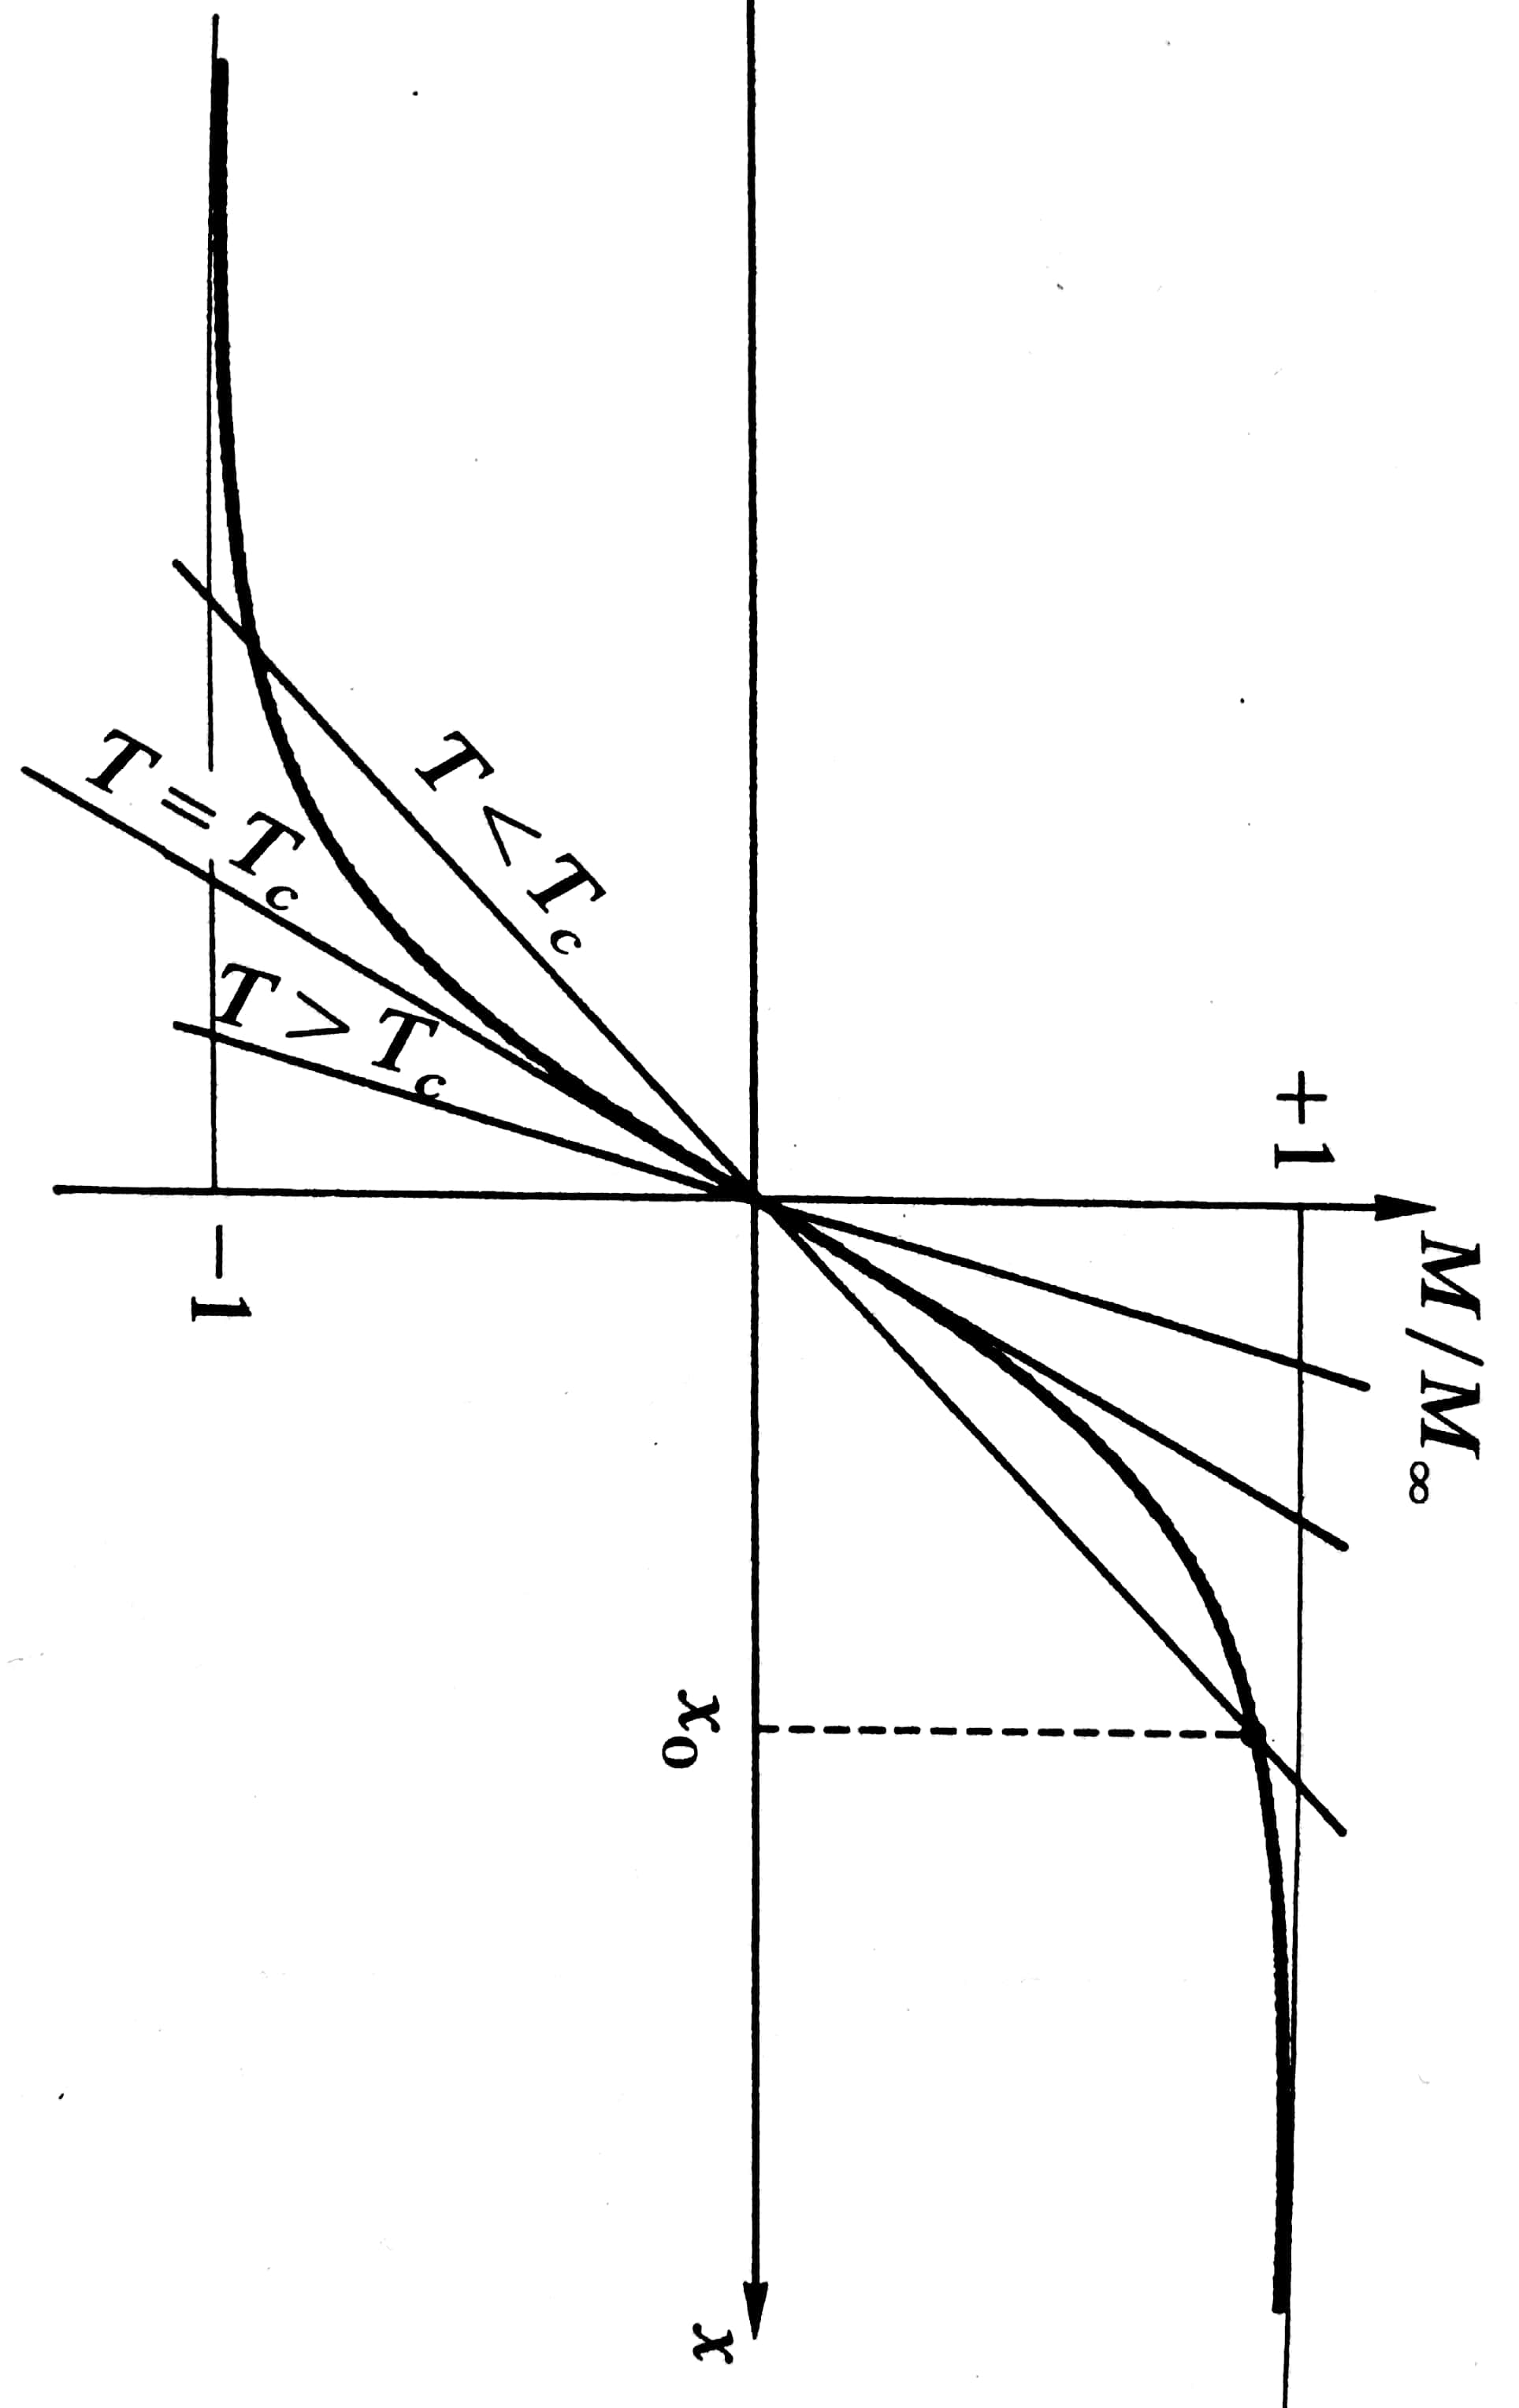
\includegraphics[width=7cm,angle=90]{Mx3}}
\end{figure}
\end{frame}

\begin{frame}
\frametitle{Énergie libre}
\begin{figure}
	\centerline{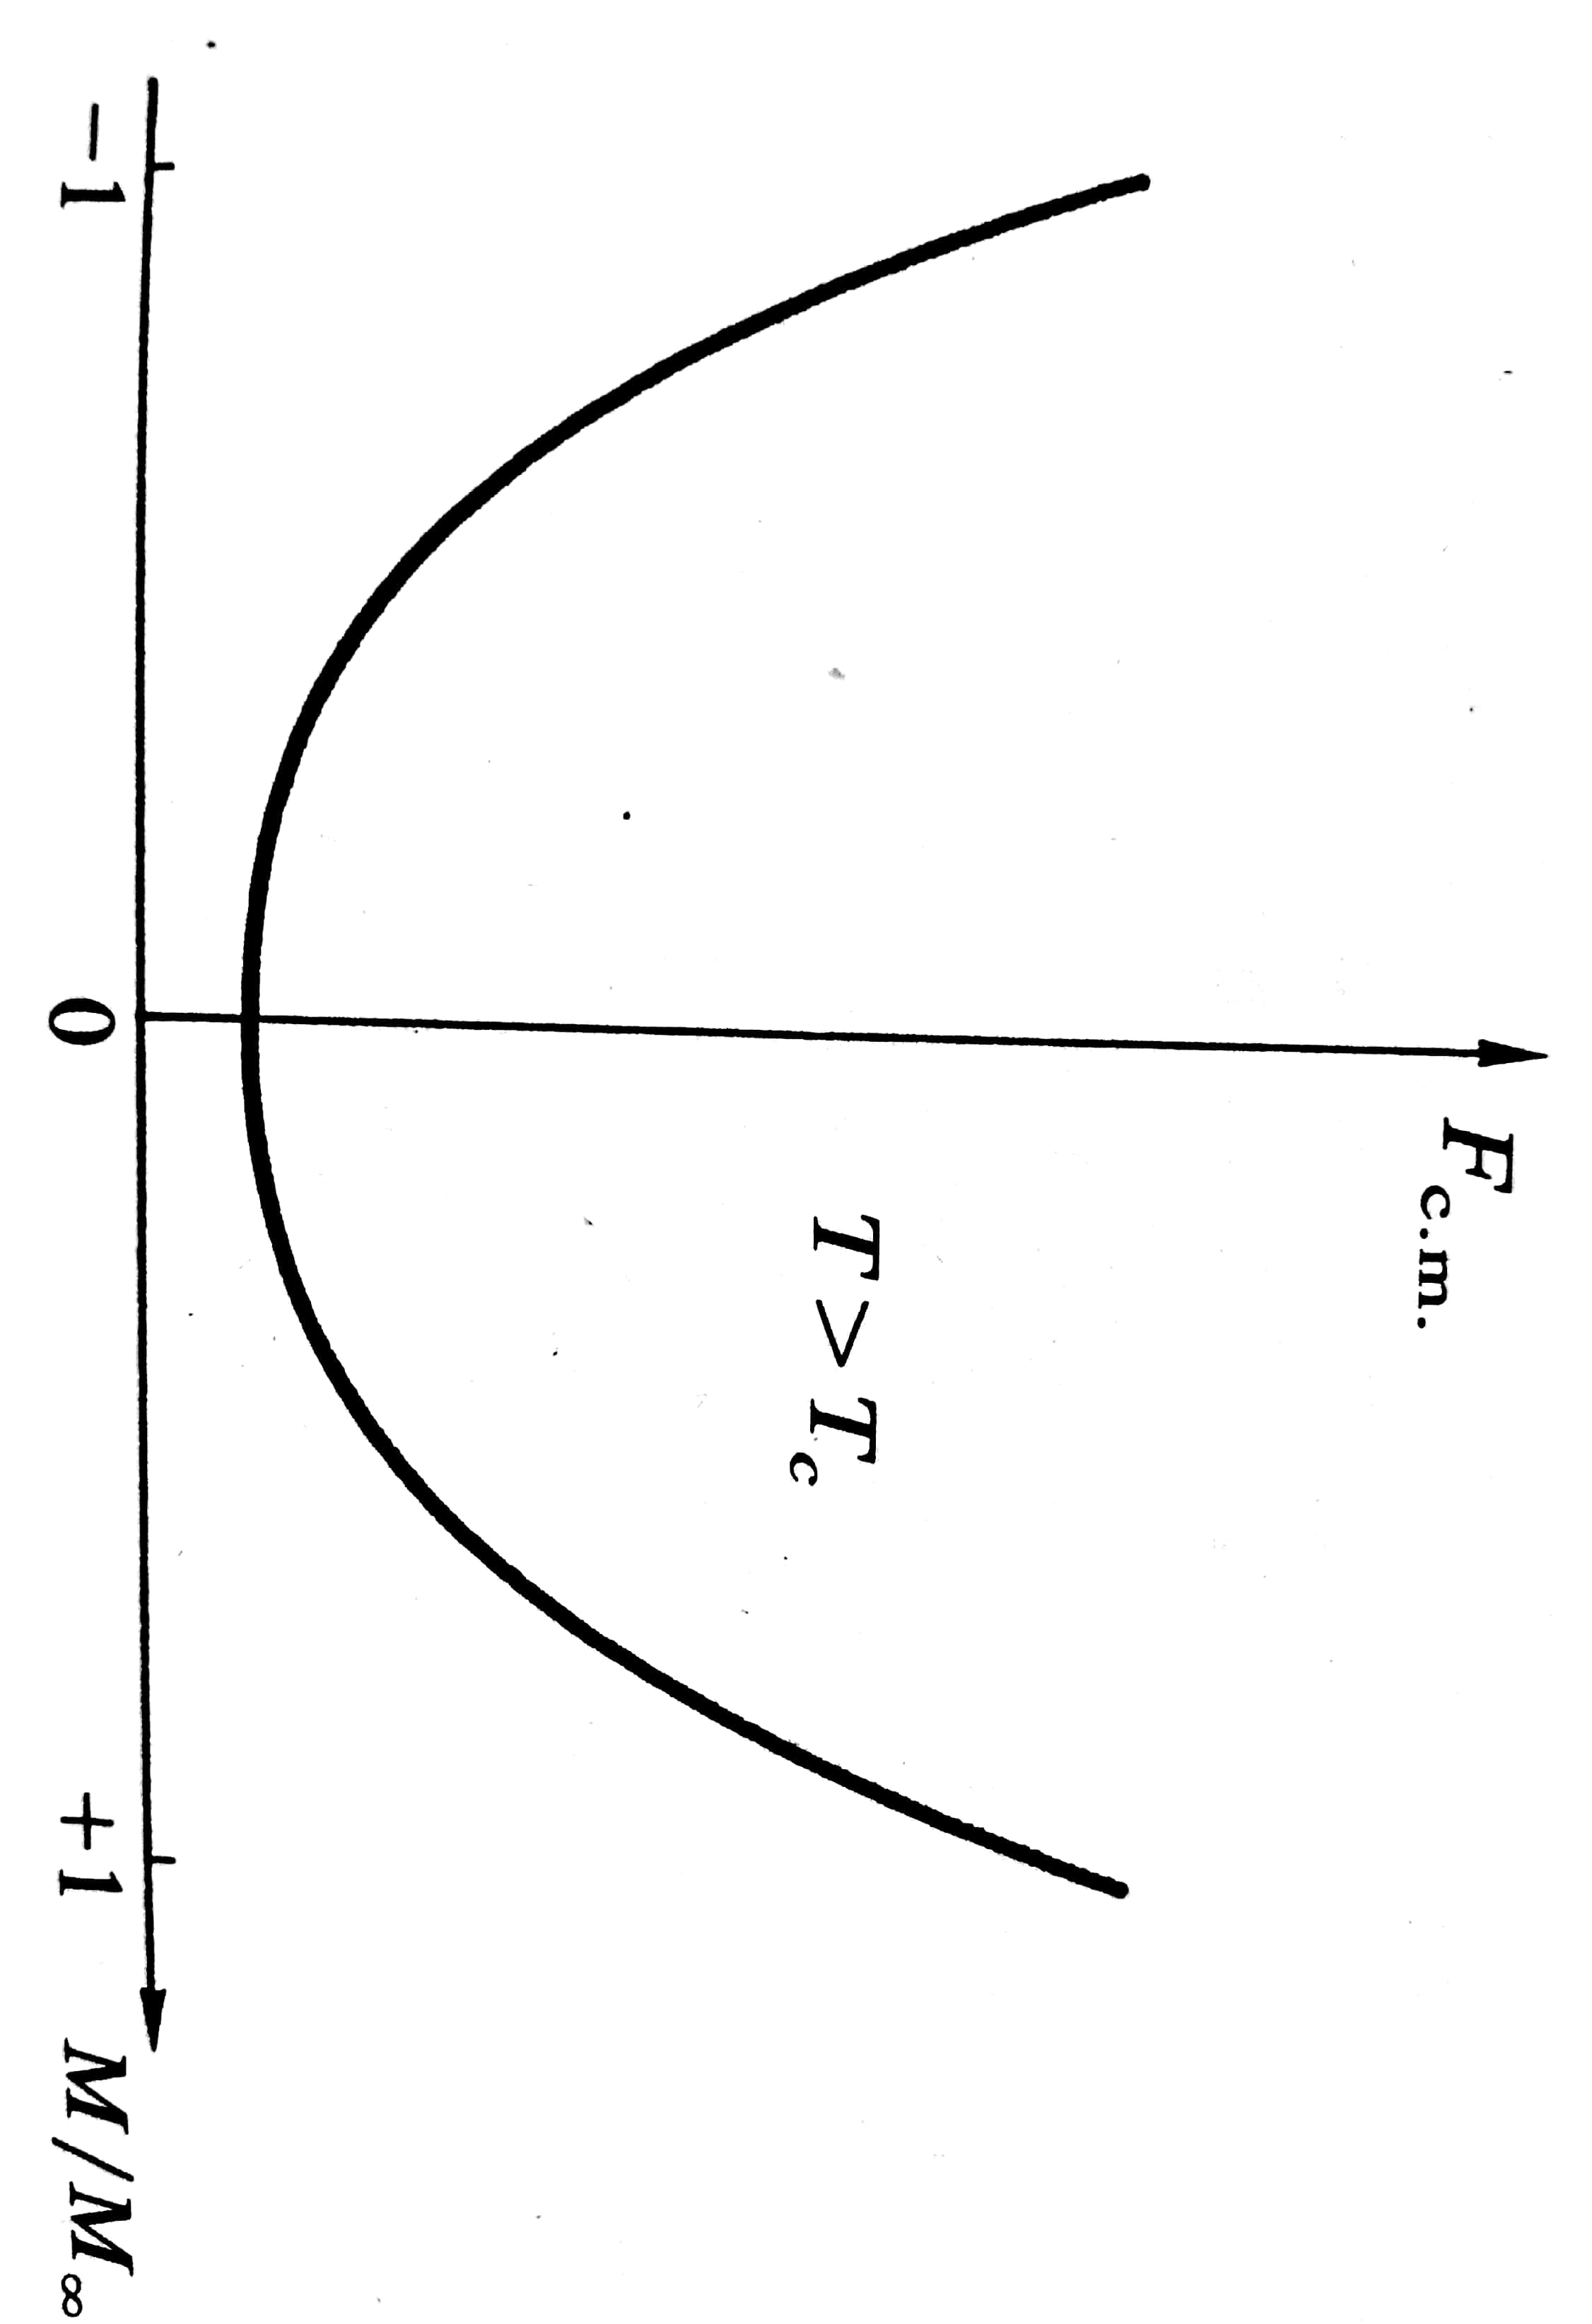
\includegraphics[width=4.2cm,angle=90]{F_T_sup_Tc}
		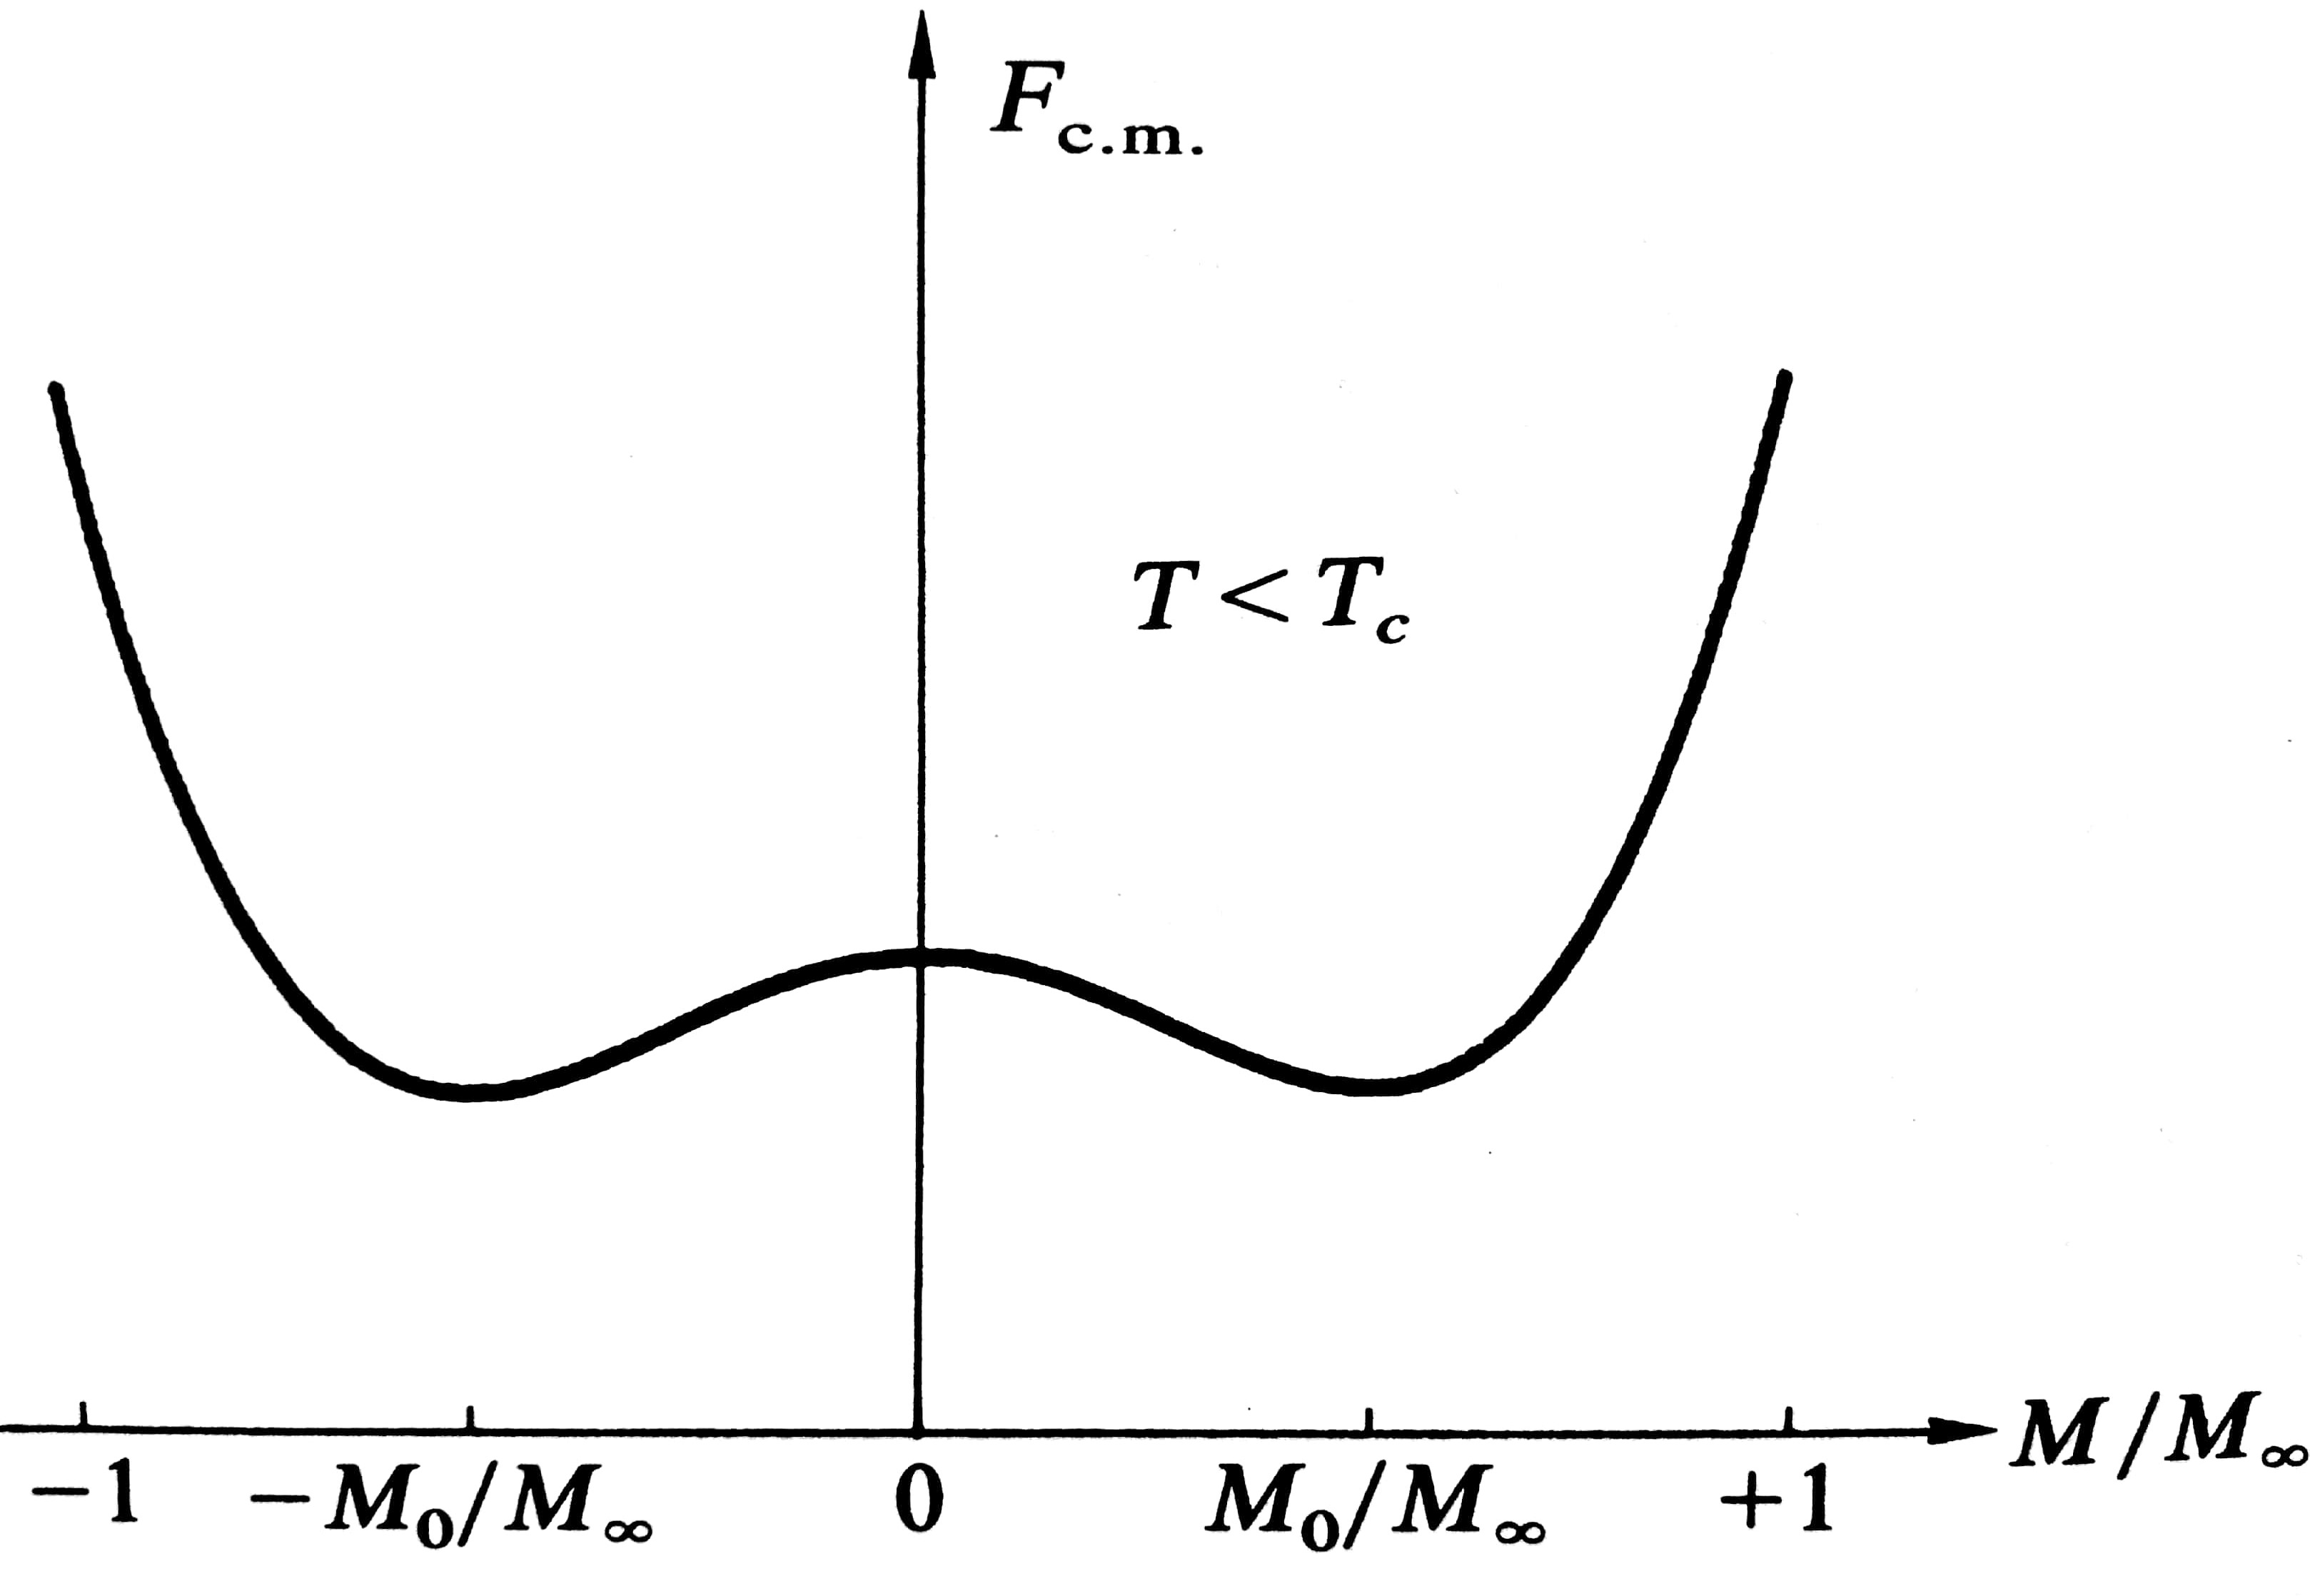
\includegraphics[width=5.8cm]{F_T_inf_Tc}}
\end{figure}
\end{frame}

\begin{frame}
\frametitle{Solution générale : $T>T_c$}
\begin{figure}
	\centerline{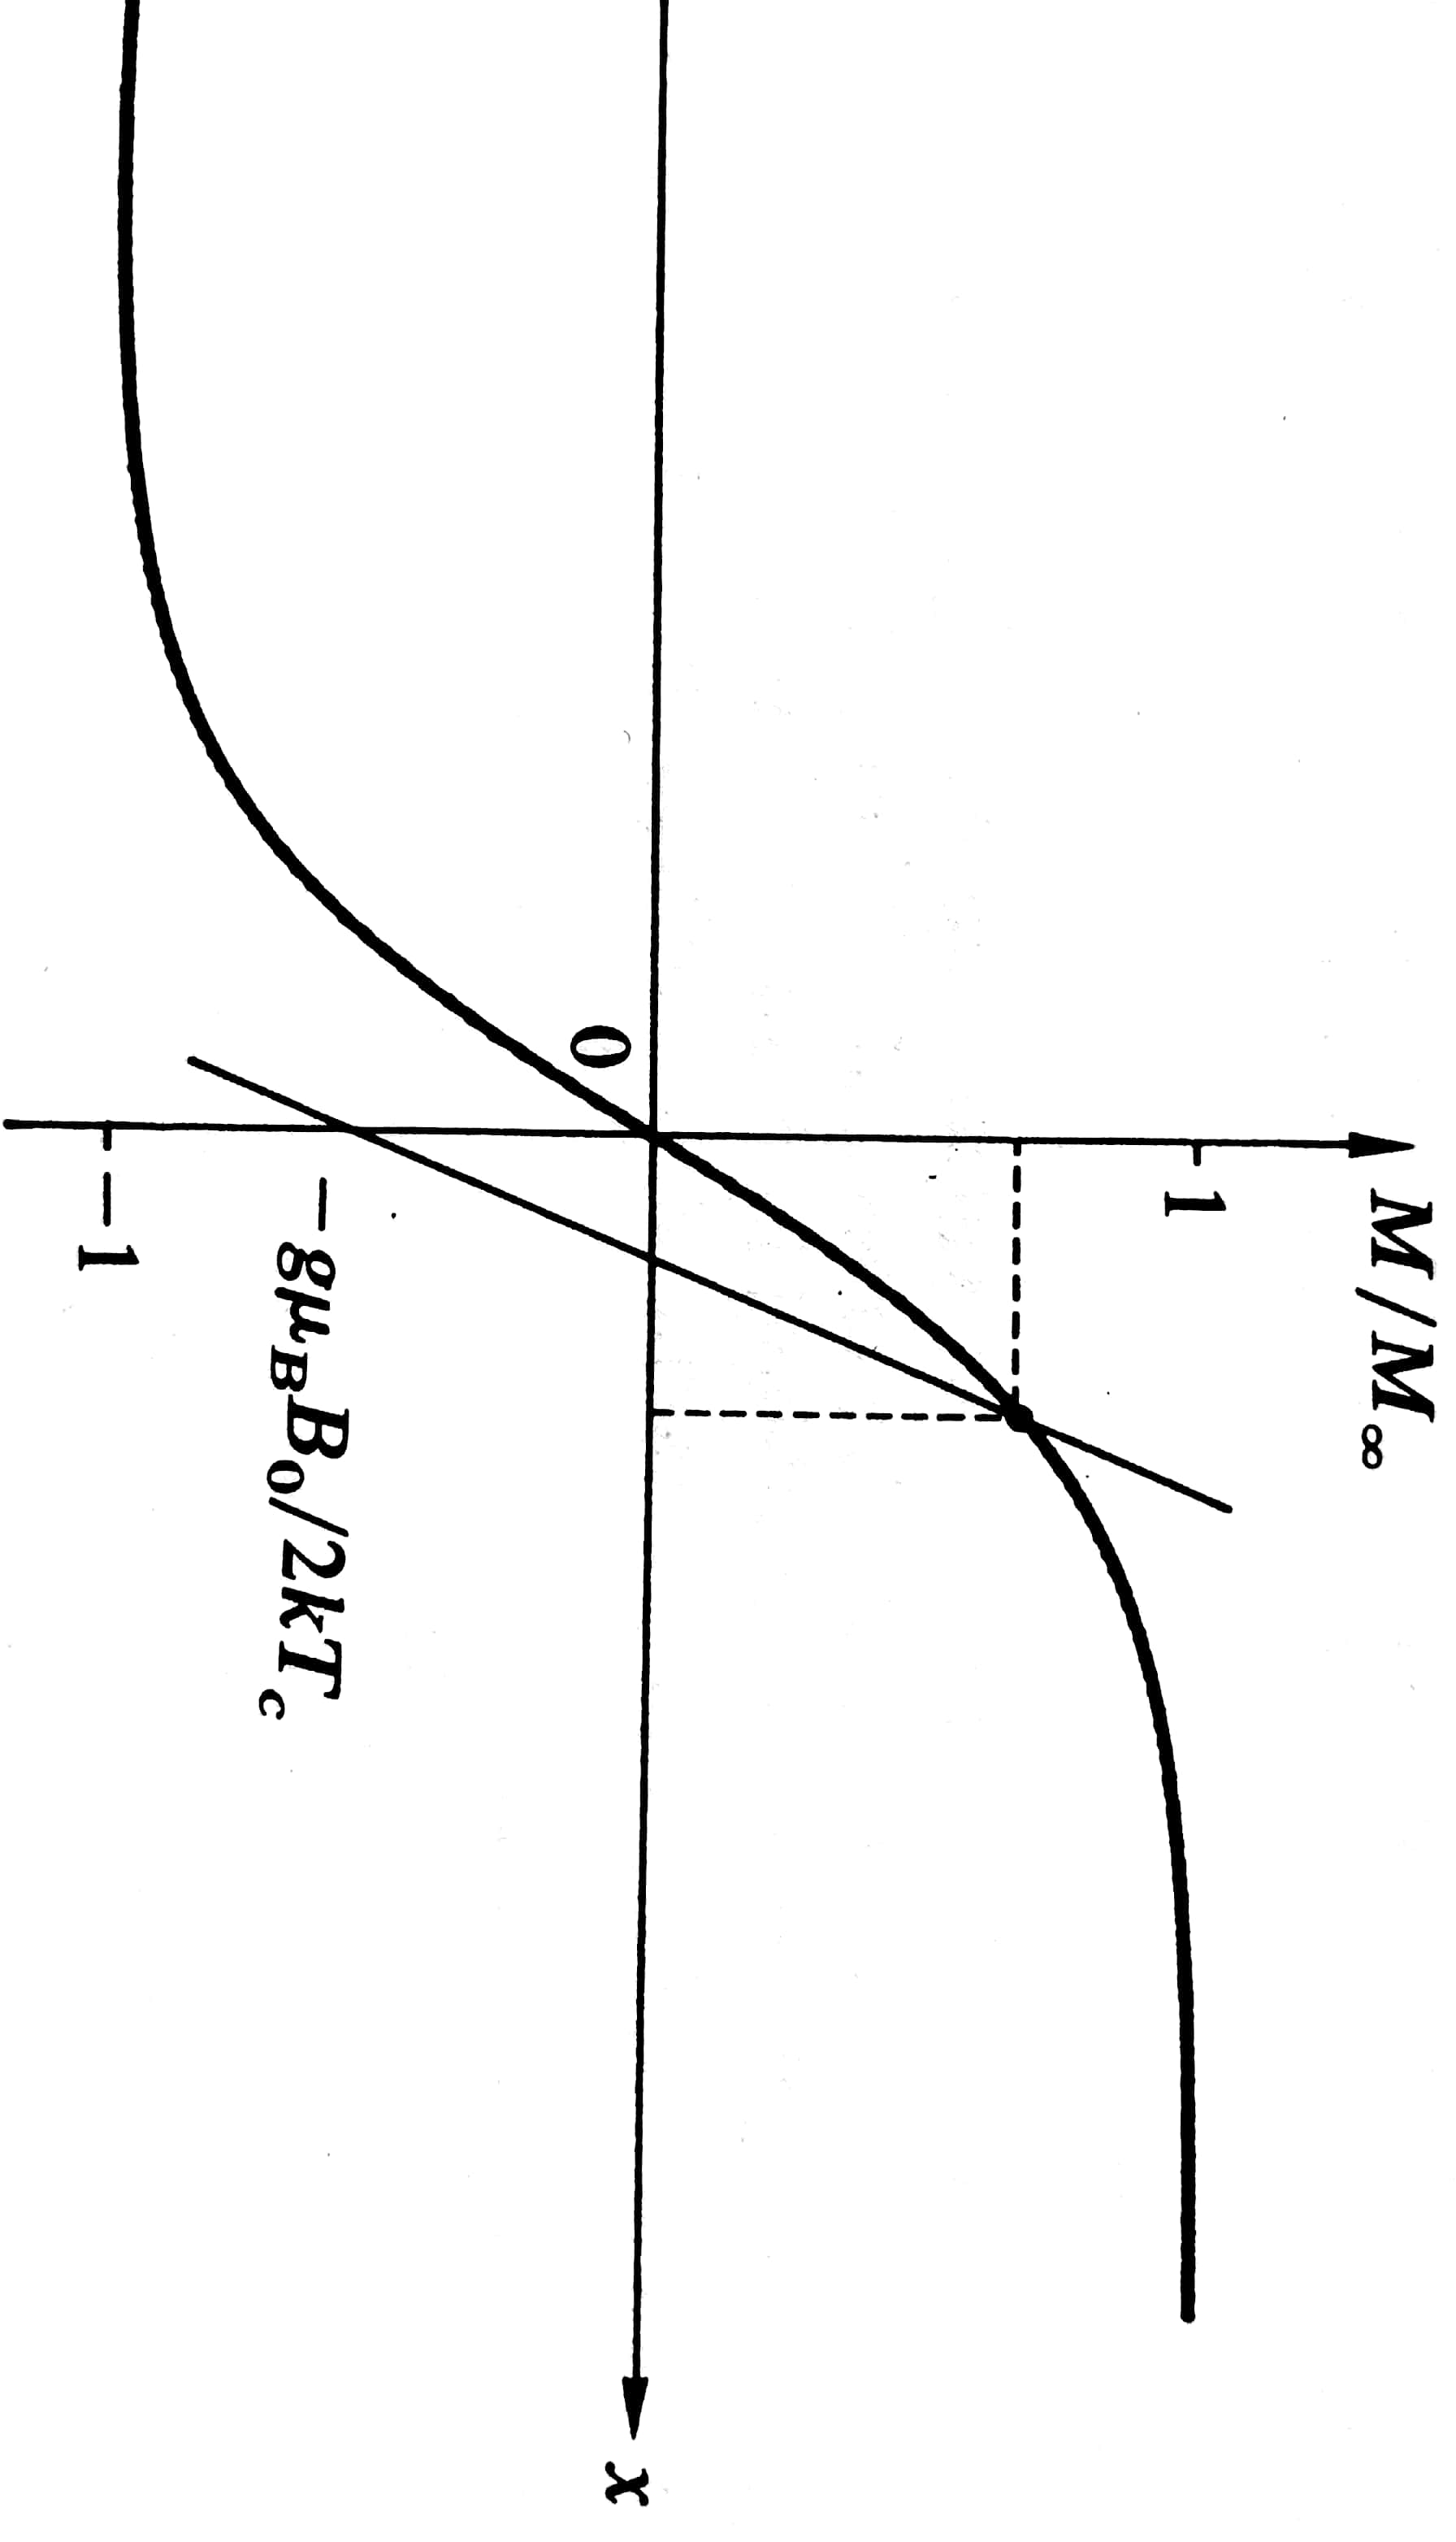
\includegraphics[width=6cm,angle=90]{Mx2}}
\end{figure}	
\end{frame}

\begin{frame}
\frametitle{Solution générale : $T<T_c$}
\begin{figure}
	\centerline{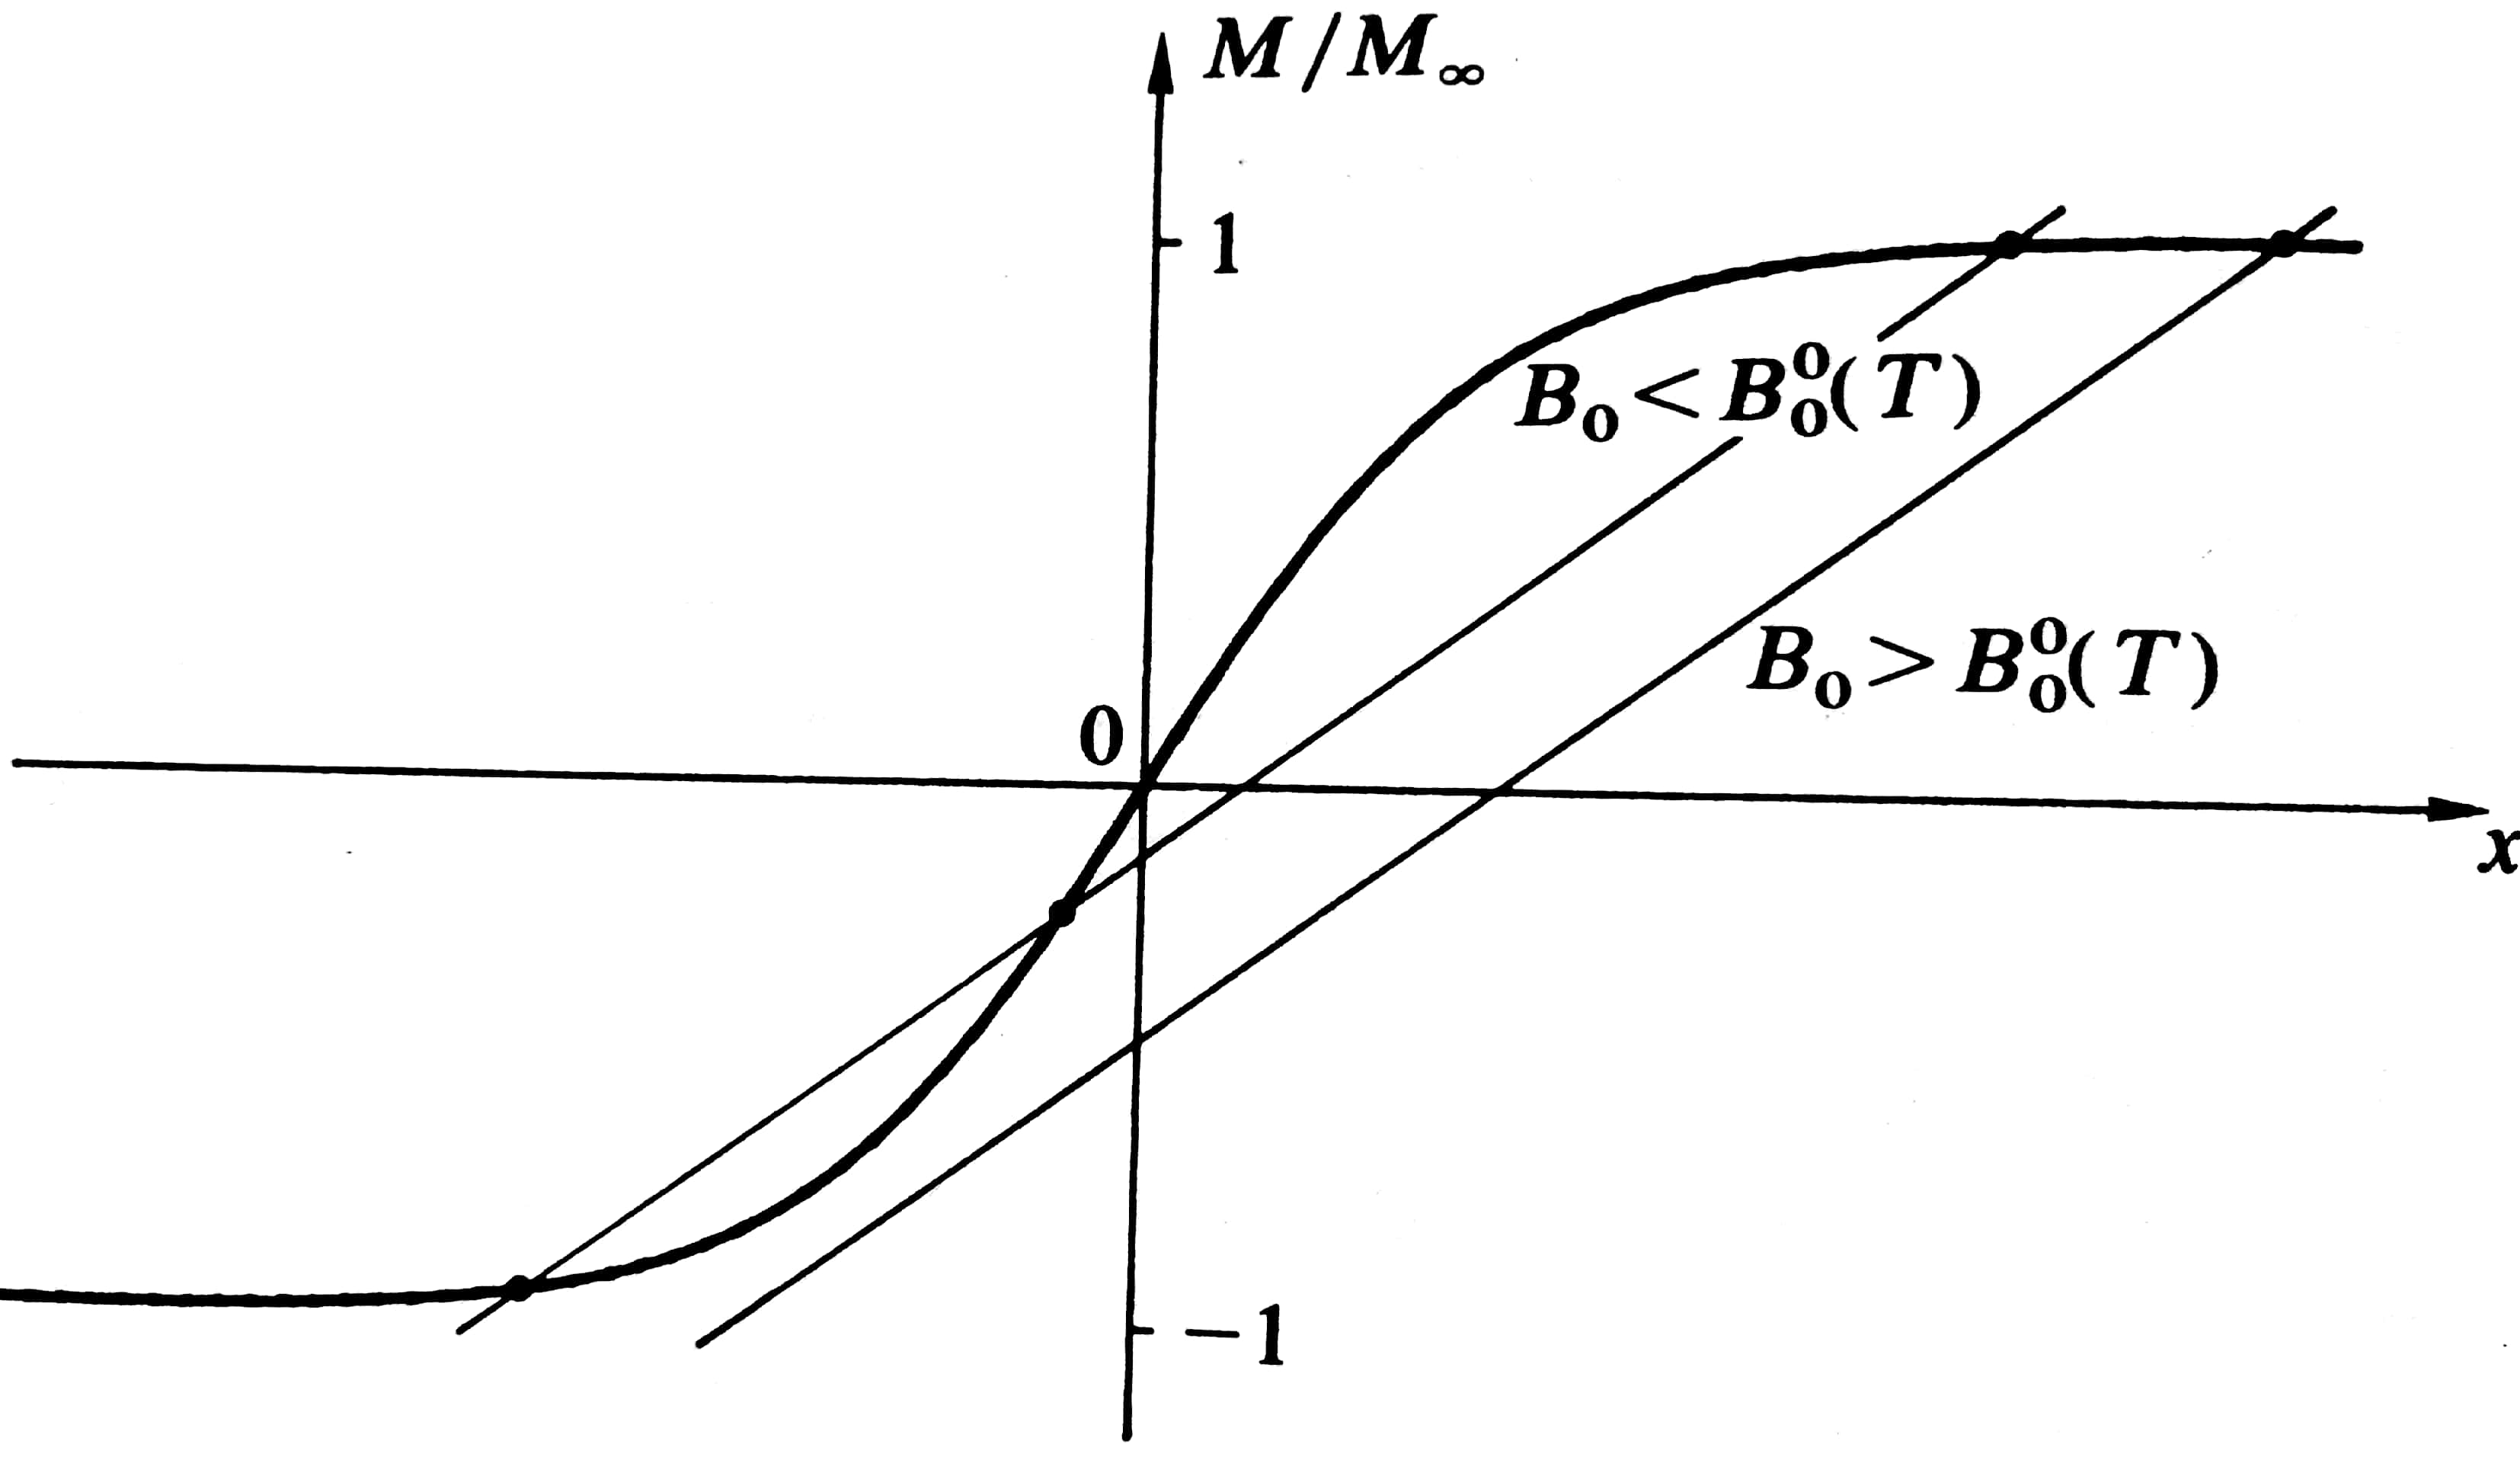
\includegraphics[width=10cm]{def_B0}}
\end{figure}
\end{frame}

\begin{frame}
\frametitle{Solution générale : énergie libre}
\begin{figure}
	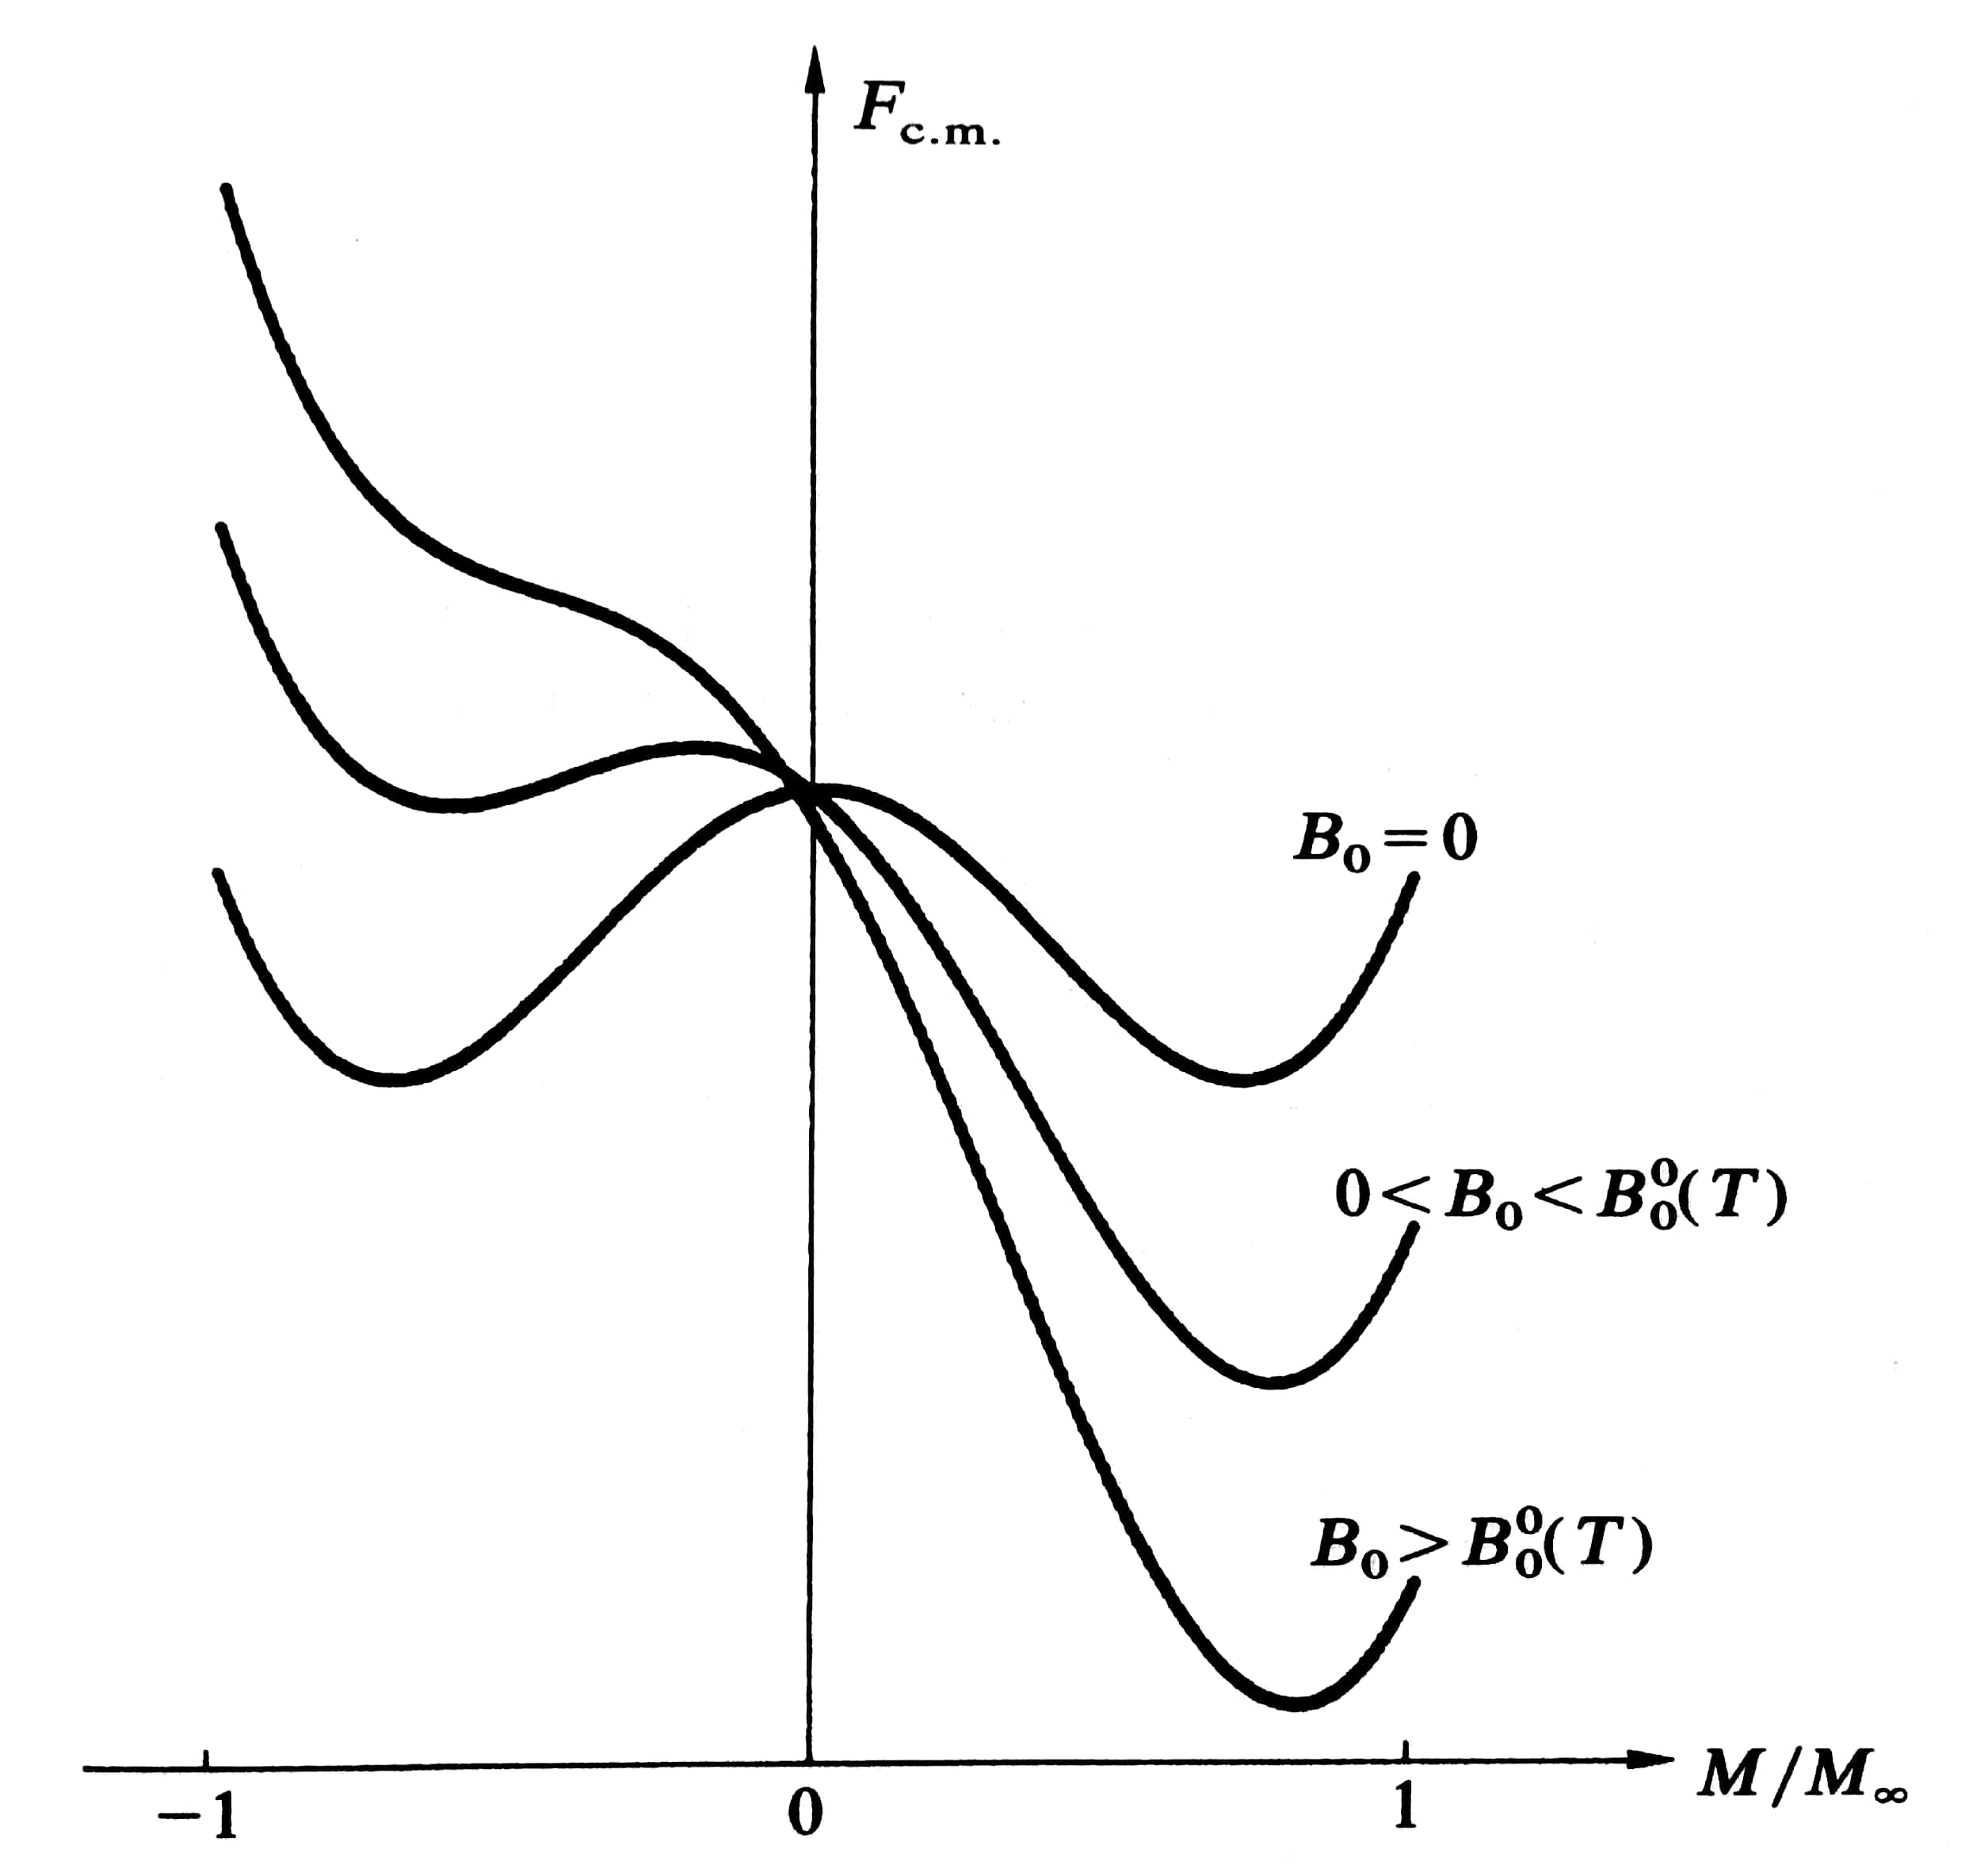
\includegraphics[width=8cm]{F_cas_general}
\end{figure}
\end{frame}

\begin{frame}
\frametitle{Comparaison avec les résultats expérimentaux}
\begin{figure}
	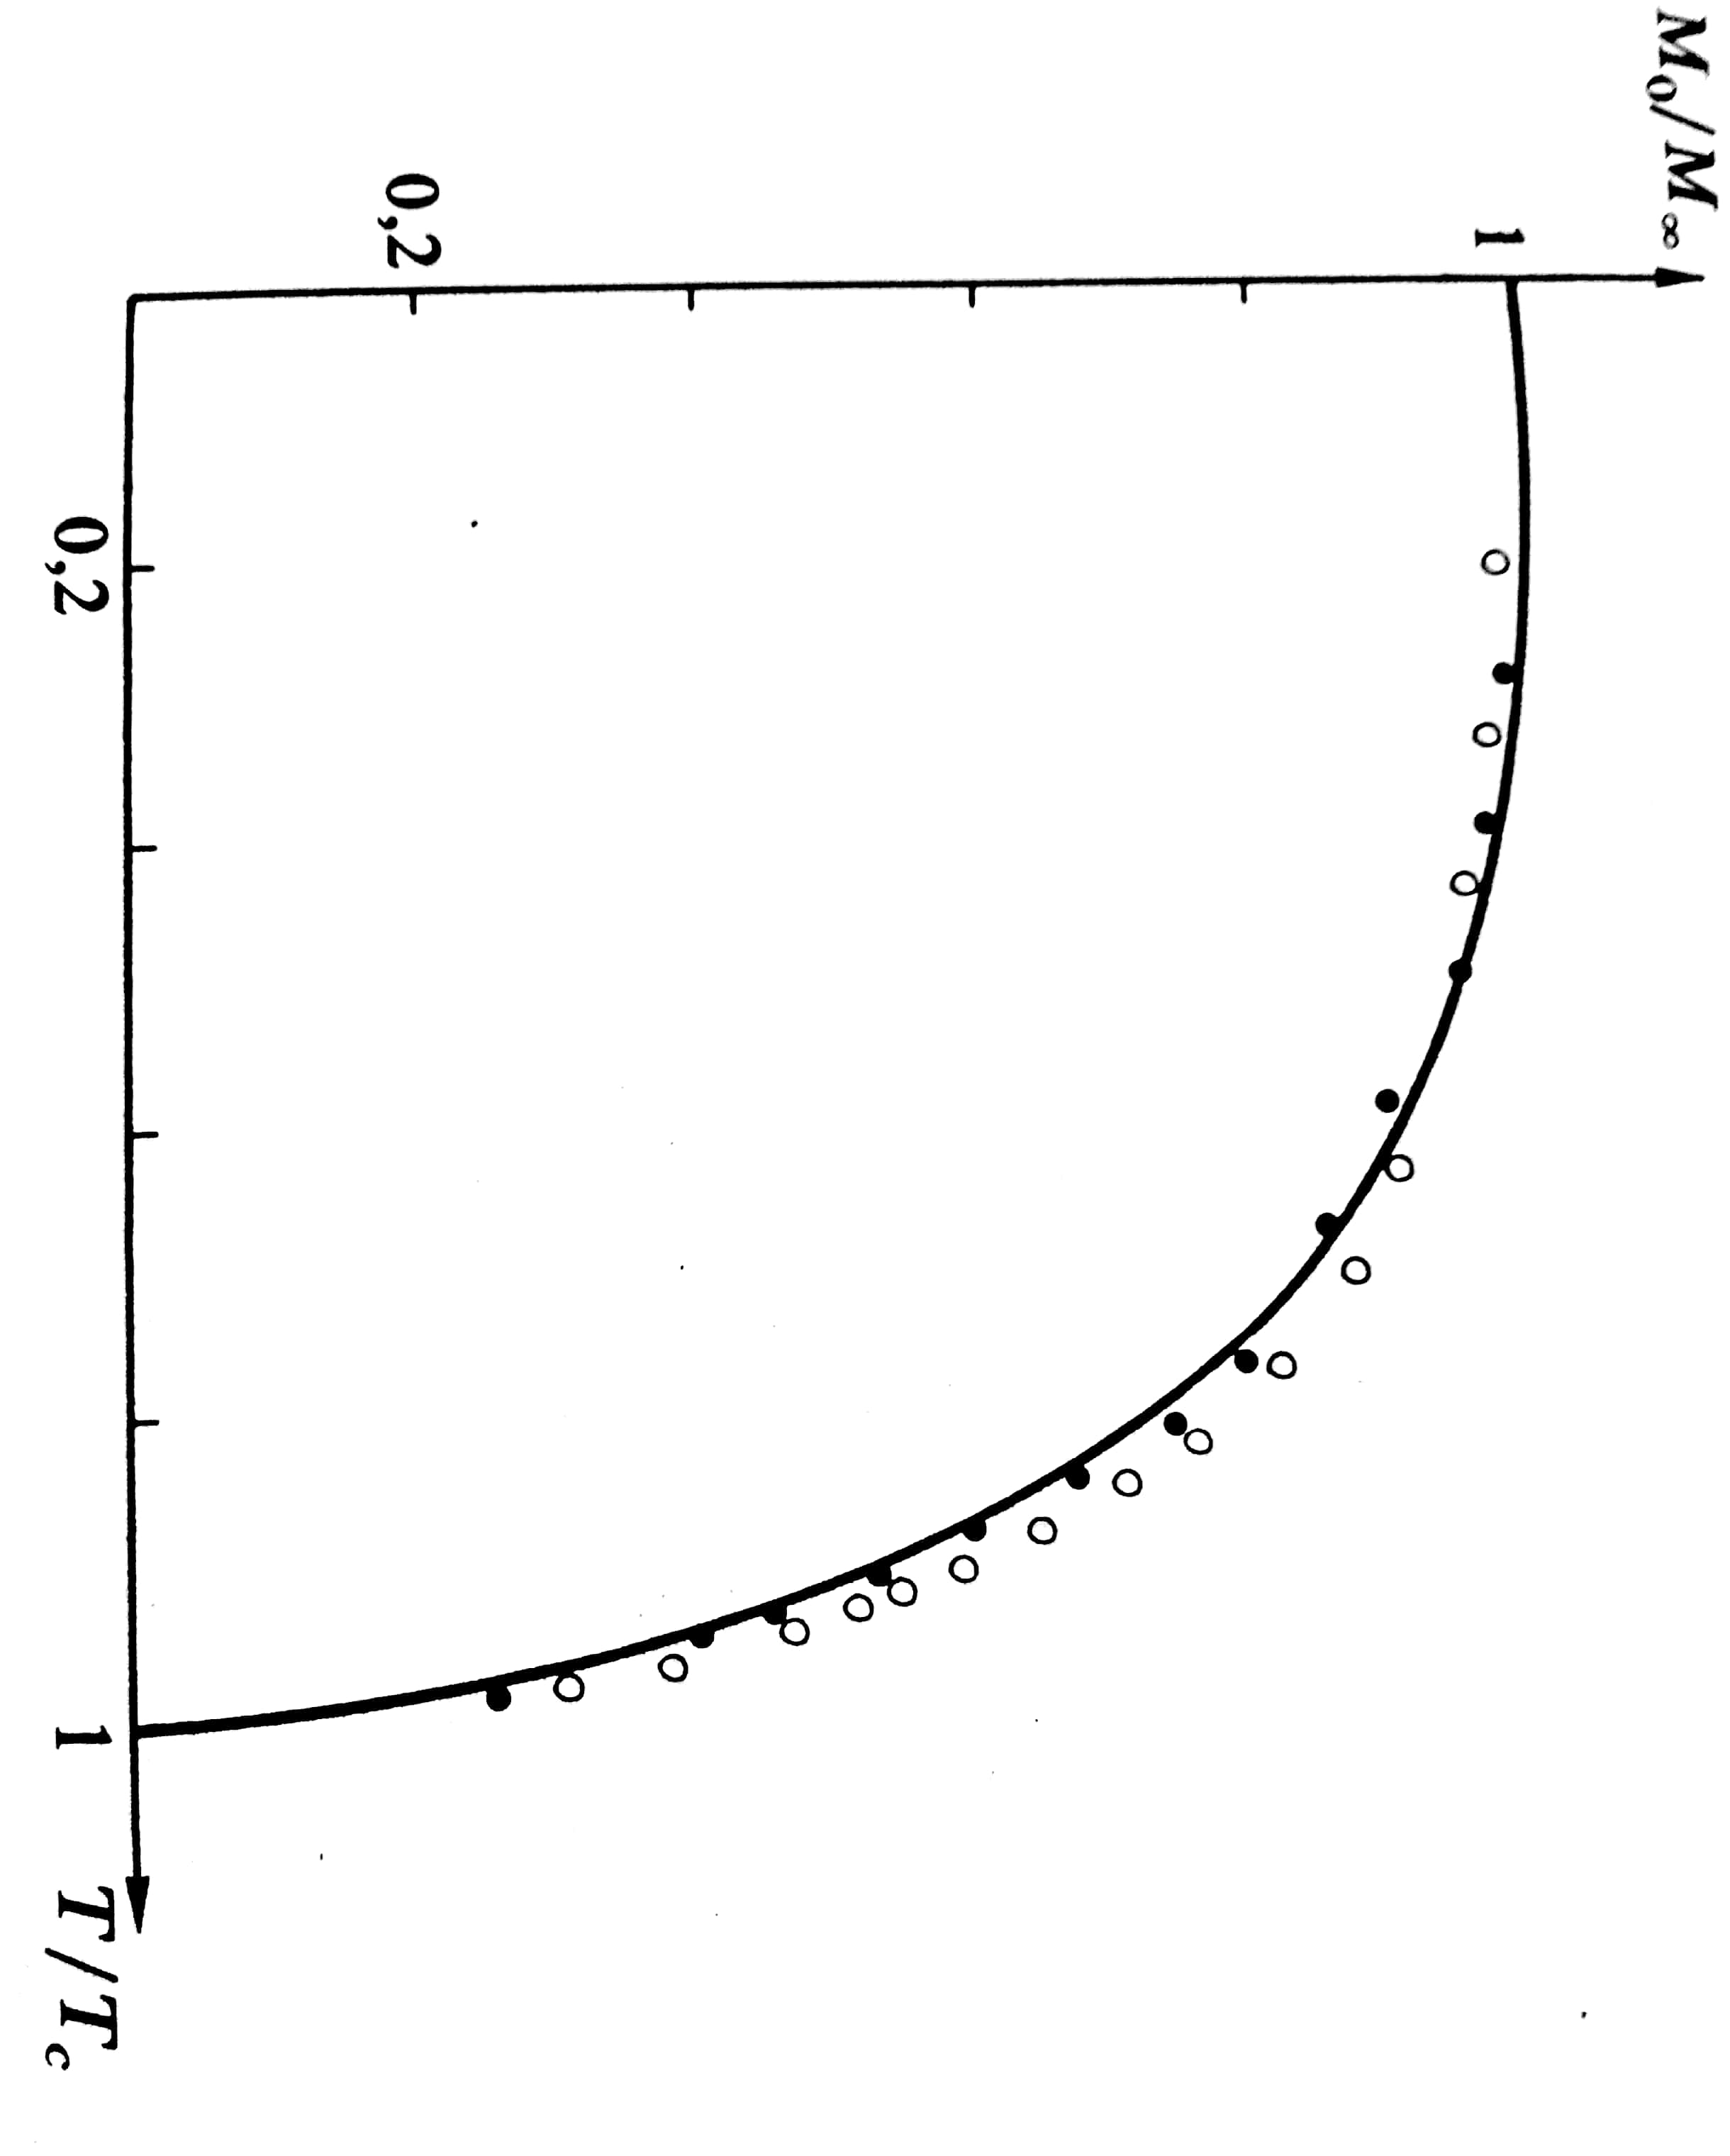
\includegraphics[width=6cm, angle=90]{comparaison}
\end{figure}
\centering{Points noirs pour le cobalt et nickel, et blancs pour le fer.}
\end{frame}

\end{document}